% Created 2022-03-18 Fri 18:44
% Intended LaTeX compiler: pdflatex
\documentclass[12pt]{article}
\usepackage[hidelinks]{hyperref}
\usepackage{amsmath}
\usepackage{amssymb}
\usepackage[left=3cm, right=3cm, top=2cm, bottom=2cm]{geometry}
\usepackage{titlesec}
\setcounter{secnumdepth}{12}
\titleformat{\paragraph}
{\normalfont\normalsize\bfseries}{\theparagraph}{1em}{}
\titlespacing*{\paragraph}
{0pt}{3.25ex plus 1ex minus .2ex}{1.5ex plus .2ex}
\usepackage{indentfirst}
\setlength{\parindent}{1em}
\setlength{\parskip}{1em}
\usepackage[export]{adjustbox}
\raggedbottom
\usepackage{float}
\clearpage
\usepackage{longtable}
\usepackage{array}
\usepackage{multirow}
\newcolumntype{C}[1]{>{\centering\arraybackslash}p{#1}}
\usepackage{gensymb}
\usepackage{graphicx}
\usepackage{tikz}
\usepackage{tikz-feynman}
\usetikzlibrary{arrows.meta, decorations.pathreplacing, decorations.markings, decorations.pathmorphing}
\tikzset{snake it/.style={decorate, decoration=snake}}
\usepackage{multicol}
\usepackage{tcolorbox}
\setlength{\columnsep}{0.1cm}
\setlength{\columnseprule}{0.5pt}
\def\columnseprulecolor{\color{white}}
\renewcommand\fbox{\fcolorbox{lightgray}{white}}
\usepackage{framed}
\usepackage{xcolor}
\usepackage{xpatch}
\let\oldsection\section
\renewcommand\section{\clearpage\oldsection}
\usepackage{fancyhdr}
\pagestyle{fancy}
\fancyhf{}
\pagestyle{fancy}
\rhead{\emph{Alexander F. Neville}}
\lhead{AQA A-Level Physics}
\rfoot{\thepage}
\lfoot{\leftmark}
\renewcommand{\headrulewidth}{1pt}
\renewcommand{\footrulewidth}{1pt}
\xpretocmd\headrule{\color{lightgray}}{}{\PatchFailed}
% \xpretocmd\footrule{\color{lightgray}}{}{\PatchFailed}
\usepackage{etoolbox}
\makeatletter
\patchcmd{\footrule}
{\if@fancyplain}
{\color{lightgray}\if@fancyplain}
{}
{}
\makeatother
\author{Alexander Neville}
\date{\today}
\title{Physics Notes}
\hypersetup{
 pdfauthor={Alexander Neville},
 pdftitle={Physics Notes},
 pdfkeywords={},
 pdfsubject={},
 pdfcreator={Emacs 27.1 (Org mode 9.6)}, 
 pdflang={English}}
\begin{document}

\maketitle
\thispagestyle{empty}
\begin{figure}[H]
\centering
% \includegraphics[width=0.9\textwidth,keepaspectratio,frame]{./images/}
\end{figure}
\newpage
%inner square side length
\def\a{3.0}
%outer square side length
\def\b{5.0}
% x displacement of back squares
\def\dx{0.8}
% y displacement of back squares
\def\dy{0.5}
\def\lx{1.0}
\def\ly{1.0}
% round corner correction
\def\dr{0.02}
\tableofcontents

\section{Particle Physics}
\label{sec:org7e61439}
\subsection{Atoms \& Nuclei}
\label{sec:org9aaff95}

An atom is composed of a positively charged, centrally located mass called the \emph{nucleus}, surrounded by negatively charged \emph{electrons}. These electrons are held in the atom by the \emph{electrostatic force of attraction} from the positive nucleus. The ratio of electron mass to nucleon mass is about \(0.0005\). Therefore the majority of an atoms mass is contained in the nucleus. The ratio of the diameter of a nucleus to the typical diameter of an atom is about \(0.000001\).


% insert table about p, n and e

\subsubsection{Isotopes}
\label{sec:orgc7453fa}

Every atom of a particular element has the same number of protons as the next. The proton number, also called the atomic number and denoted with the letter \(Z\), identifies particular atoms. Atoms of a certain element can have \textbf{different} neutron totals. These atoms share the same proton number so they are of the same element and are \emph{isotopes} of that element. The total number of nucleons (neutrons and protons) is denoted with the letter \(A\) and sometimes called the mass number. The number of neutrons in a nucleus is equal to \(A - Z\). An unspecified element may be represented with the notation \(^{A}_{Z}X\) where the mass number is displayed above the proton number. Each type of a nucleus of element \(X\) is called a \emph{nuclide}.

\subsubsection{Specific Charge}
\label{sec:org5106799}

The specific charge of a charged particle is the total charge over its mass. The specific charge for a nucleus, nucleon, electron, ion or other particle can all be calculated.

\subsubsection{Strong Nuclear Force}
\label{sec:org9c981e8}

Protons in a nucleus experience repulsion from one another due to their like charge. A separate force is required to oppose the electrostatic force between protons and prevent the disintegration of nuclei. This force is known as the \emph{Strong Nuclear Force}.

\begin{itemize}
\item The range of the strong force is limited to about \(3-4fm\), the typical diameter of an a small nucleus. The range of the electrostatic force is unlimited, but decreases with distance.

\item The effect felt between a neutron and a proton is the same as the force experienced between any nucleon combination.

\item The strong force is repulsive below \(0.5fm\) and attractive from this point to the extent of its range. This prevents nucleons being pushed into each other and hence the collapse of a nucleus.
\end{itemize}


% graph of force against seperation

\subsubsection{Force Carriers}
\label{sec:orge2187cd}

Forces acting on objects cause a change in momentum according to \(F = mv/t\). This is observed when two charged particles approach one another. For example, the electromagnetic force between particles is due to an exchange particle, in this case a \emph{virtual photon}.


\begin{figure}[H]
\centering
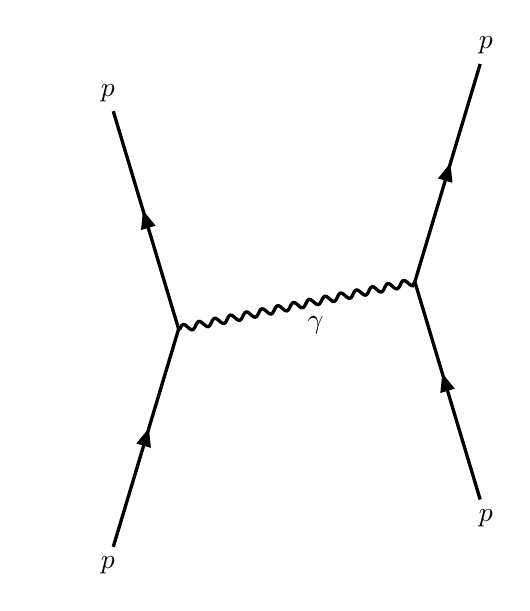
\begin{tikzpicture}[x=30mm, y=30mm]
\begin{feynman}
    \vertex (i1) {};
    \vertex[right=.3 of i1] (i3) {\(p\)};
    \vertex[above=2 of i1] (f1) {};
    \vertex[right=.3 of f1] (f3) {\(p\)};
    \vertex[above=1 of i3] (a);
    \vertex[right=.15 of a] (b);
    \vertex[right=.15 of b] (c);
    \vertex at ($(c) + (1,.2)$) (d);
    \vertex at ($(d) + (.3, 1)$) (f4) {\(p\)};
    \vertex at ($(d) + (.3,-1)$) (f5) {\(p\)};
\diagram*{
    (i3) -- [fermion, very thick] (c) -- [fermion, very thick] (f3),
    (c) -- [boson, edge label'=\(\gamma \), very thick] (d),
    (d) -- [anti fermion, very thick] (f5),
    (d) -- [fermion, very thick] (f4),
};
% \draw[-stealth] (-.4,-.4) -- (-.4,2.2);
% \node at (-.4,2.3) {\(t\)};
\end{feynman}
\end{tikzpicture}
\caption{Electromagnetic force between two protons}
\end{figure}

\subsubsection{Weak Interaction}
\label{sec:org2c08a6d}

The \emph{Weak Nuclear Force} causes some nuclear changes, such as beta emission. It is so called as its strength is less than the strong nuclear force, preventing the disintegration of stable nuclei. The exchange particle of the \emph{weak interaction} is the \emph{W boson}. These are charged particles with a very short range and non-zero rest mass.

\subsection{Radioactive Decay}
\label{sec:org165dc64}

Naturally occurring radioactive isotopes emit three types of radiation:

\begin{enumerate}
\item Alpha: \(^4_2\alpha\)
\item Beta: \(^{ \text{ } \text{ } 0}_{-1}\beta^-\) / \(^{0}_{1}\beta^+\)
\item Gamma: \(\gamma\)
\end{enumerate}

\subsubsection{Alpha Emission}
\label{sec:org3e42432}

An \(\alpha\) particle is composed of two neutrons and two protons. The product nucleus \(Y\), after \(\alpha\) emission has taken place, is a of a different, lighter element.

\[^A_ZX \rightarrow \text{} ^4_2\alpha + \text{} ^{A-4}_{Z-2}Y\]

\subsubsection{Beta Minus Decay}
\label{sec:org0b5c379}

A \(\beta^-\) particle is an electron. During \(\beta^-\) emission, a neutron in a neutron-rich nucleus decays into a proton. The underlying change is the conversion of a \emph{down quark} into an \emph{up quark}. Along with a fast-moving electron, an \emph{electron antineutrino} is produced.

\[^A_ZX \rightarrow \text{} ^{ \text{ } \text{ }0}_{-1}\beta + \text{} ^{\text{ } \text{ }A}_{Z+1}Y + \bar{\nu}_e\]


\begin{figure}[H]
\centering
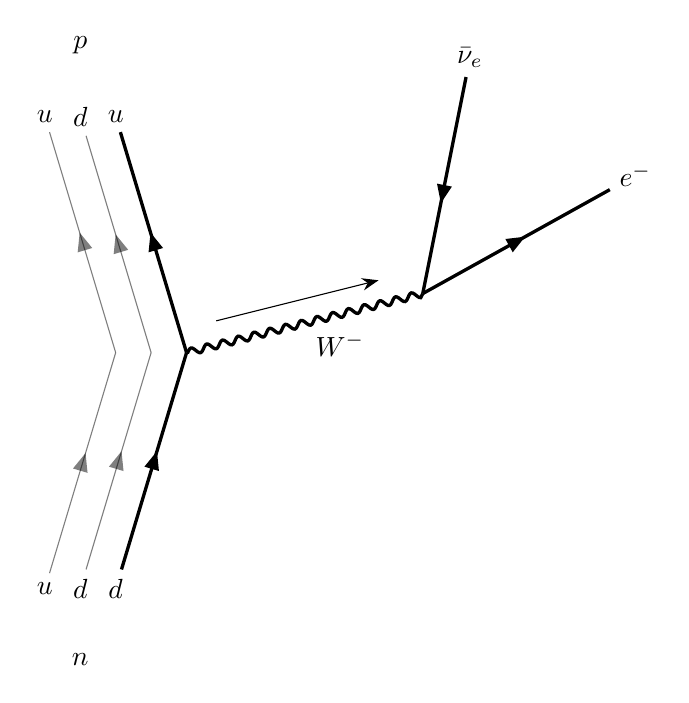
\begin{tikzpicture}[x=30mm, y=30mm]
\begin{feynman}
    \vertex (i1) {\(u\)};
    \vertex[right=.15 of i1] (i2) {\(d\)};
    \vertex[right=.15 of i2] (i3) {\(d\)};
    \vertex[below=.3 of i2] (n) {\(n\)};
    \vertex[above=2 of i1] (f1) {\(u\)};
    \vertex[right=.15 of f1] (f2) {\(d\)};
    \vertex[right=.15 of f2] (f3) {\(u\)};
    \vertex[above=.3 of f2] (p) {\(p\)};
    \vertex[above=1 of i3] (a);
    \vertex[right=.15 of a] (b);
    \vertex[right=.15 of b] (c);
    \vertex at ($(c) + (1,.25)$) (d);
    \vertex at ($(d) + (.2, 1)$) (f4) {\(\bar{\nu}_e\)};
    \vertex at ($(d) + (.9,.5)$) (f5) {\(e^-\)};
\diagram*{
    (i1) -- [fermion, opacity=0.5] (a) -- [fermion, opacity=0.5] (f1),
    (i2) -- [fermion, opacity=0.5] (b) -- [fermion, opacity=0.5] (f2),
    (i3) -- [fermion, very thick] (c) -- [fermion, very thick] (f3),
    (c) -- [boson, edge label'=\(W^-\), momentum, very thick] (d),
    (d) -- [fermion, very thick] (f5),
    (d) -- [anti fermion, very thick] (f4),
};
% \draw[-stealth] (-.4,-.4) -- (-.4,2.2);
% \node at (-.4,2.3) {\(t\)};
\end{feynman}
\end{tikzpicture}
\caption{Beta minus decay}
\end{figure}

\subsubsection{Beta Plus Decay}
\label{sec:orga768c93}

A \(\beta^+\) particle is a positron. During \(\beta^+\) emission, a proton in a proton-rich nucleus decays into a neutron. The underlying change is the conversion of an \emph{up quark} into an \emph{down quark}. Along with a fast-moving positron, an \emph{electron neutrino} is produced.

\[^A_ZX \rightarrow \text{} ^{ \text{ } \text{ }0}_{+1}\beta + \text{} ^{\text{ } \text{ }A}_{Z-1}Y + \nu_e\]


\begin{figure}[H]
\centering
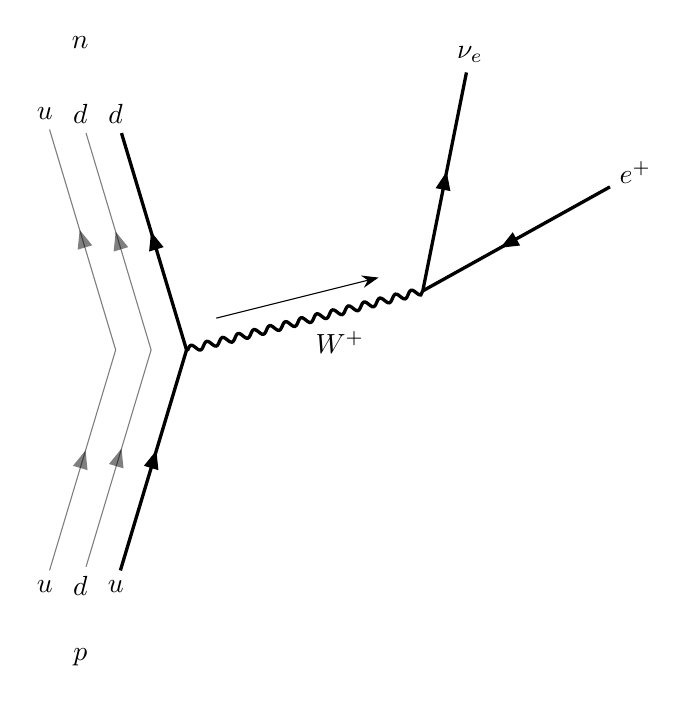
\begin{tikzpicture}[x=30mm, y=30mm]
\begin{feynman}
    \vertex (i1) {\(u\)};
    \vertex[right=.15 of i1] (i2) {\(d\)};
    \vertex[right=.15 of i2] (i3) {\(u\)};
    \vertex[below=.3 of i2] (n) {\(p\)};
    \vertex[above=2 of i1] (f1) {\(u\)};
    \vertex[right=.15 of f1] (f2) {\(d\)};
    \vertex[right=.15 of f2] (f3) {\(d\)};
    \vertex[above=.3 of f2] (p) {\(n\)};
    \vertex[above=1 of i3] (a);
    \vertex[right=.15 of a] (b);
    \vertex[right=.15 of b] (c);
    \vertex at ($(c) + (1,.25)$) (d);
    \vertex at ($(d) + (.2, 1)$) (f4) {\(\nu_e\)};
    \vertex at ($(d) + (.9,.5)$) (f5) {\(e^+\)};
\diagram*{
    (i1) -- [fermion, opacity=0.5] (a) -- [fermion, opacity=0.5] (f1),
    (i2) -- [fermion, opacity=0.5] (b) -- [fermion, opacity=0.5] (f2),
    (i3) -- [fermion, very thick] (c) -- [fermion, very thick] (f3),
    (c) -- [boson, edge label'=\(W^+\), momentum, very thick] (d),
    (d) -- [anti fermion, very thick] (f5),
    (d) -- [fermion, very thick] (f4),
};
% \draw[-stealth] (-.4,-.4) -- (-.4,2.2);
% \node at (-.4,2.3) {\(t\)};
\end{feynman}
\end{tikzpicture}
\caption{Beta plus decay}
\end{figure}

\subsubsection{Electron Capture}
\label{sec:orge09b381}

A proton-rich nucleus could also undergo \emph{electron capture}. In this type of decay a proton changes into a neutron after capturing an inner shell electron. The nature of the \emph{W boson} is not significant/distinguishable.

\[^A_ZX + ^{ \text{ } \text{ }0}_{-1}\beta \rightarrow \text{} ^{\text{ } \text{ }A}_{Z-1}Y + \nu_e\]

\begin{figure}[H]
\centering
\begin{minipage}{.45\textwidth}
    \centering
    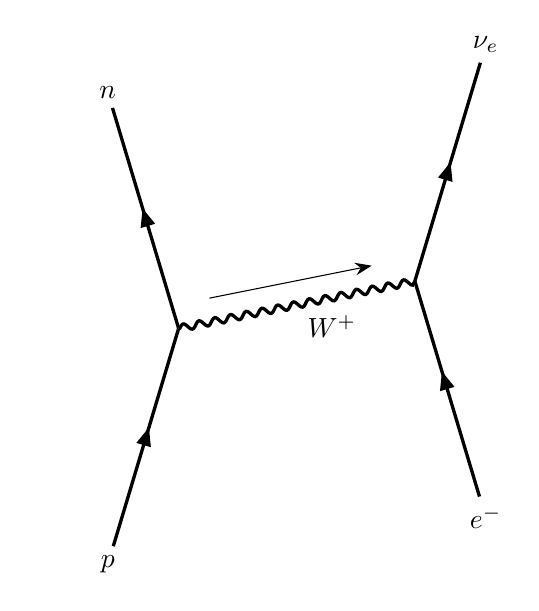
\begin{tikzpicture}[x=30mm, y=30mm]
    \begin{feynman}
        \vertex (i1) {};
        \vertex[right=.3 of i1] (i3) {\(p\)};
        \vertex[above=2 of i1] (f1) {};
        \vertex[right=.3 of f1] (f3) {\(n\)};
        \vertex[above=1 of i3] (a);
        \vertex[right=.15 of a] (b);
        \vertex[right=.15 of b] (c);
        \vertex at ($(c) + (1,.2)$) (d);
        \vertex at ($(d) + (.3, 1)$) (f4) {\(\nu_e\)};
        \vertex at ($(d) + (.3,-1)$) (f5) {\(e^-\)};
    \diagram*{
        (i3) -- [fermion, very thick] (c) -- [fermion, very thick] (f3),
        (c) -- [boson, edge label'=\(W^+ \), momentum, very thick] (d),
        (d) -- [anti fermion, very thick] (f5),
        (d) -- [fermion, very thick] (f4),
    };
    % \draw[-stealth] (-.4,-.4) -- (-.4,2.2);
    % \node at (-.4,2.3) {\(t\)};
    \end{feynman}
    \end{tikzpicture}
\end{minipage}
\begin{minipage}{.45\textwidth}
  \centering
  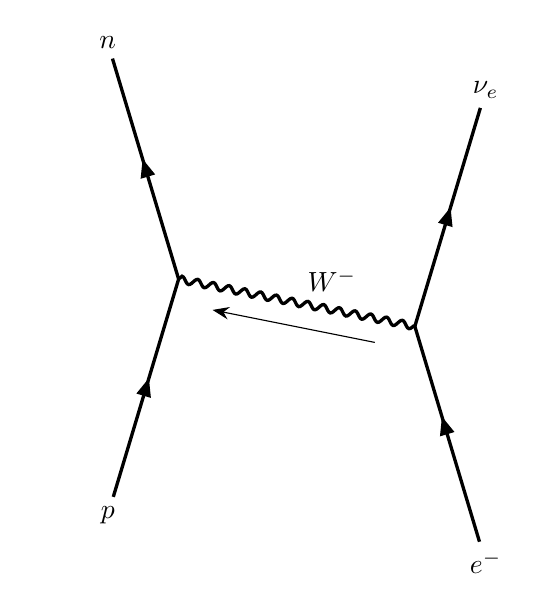
\begin{tikzpicture}[x=30mm, y=30mm]
    \begin{feynman}
        \vertex (i1) {};
        \vertex[right=.3 of i1] (i3) {\(p\)};
        \vertex[above=2 of i1] (f1) {};
        \vertex[right=.3 of f1] (f3) {\(n\)};
        \vertex[above=1 of i3] (a);
        \vertex[right=.15 of a] (b);
        \vertex[right=.15 of b] (c);
        \vertex at ($(c) + (1,-.2)$) (d);
        \vertex at ($(d) + (.3, 1)$) (f4) {\(\nu_e\)};
        \vertex at ($(d) + (.3,-1)$) (f5) {\(e^-\)};
    \diagram*{
        (i3) -- [fermion, very thick] (c) -- [fermion, very thick] (f3),
        (d) -- [boson, edge label'=\(W^- \), momentum, very thick] (c),
        (d) -- [anti fermion, very thick] (f5),
        (d) -- [fermion, very thick] (f4),
    };
    % \draw[-stealth] (-.4,-.4) -- (-.4,2.2);
    % \node at (-.4,2.3) {\(t\)};
    \end{feynman}
    \end{tikzpicture}
\end{minipage}

\caption{Electron capture}
\end{figure}

\subsubsection{Gamma Emission}
\label{sec:org7c0cbe0}

Gamma radiation is emitted by an unstable nucleus. This type of emission is pure energy with no mass and no charge. There is no change to the number of nucleons in the nucleus when a \(\gamma\) photon is emitted. This type of emission usually happens if the nucleus is in an excited state after one of the previous types of emission.

\subsection{Particles \& Antiparticles}
\label{sec:org5aa53d4}

For each type of particle, there is a corresponding \emph{antiparticle} which, in a collision event, can release the rest energy of the two particles combined. For any particle, its antiparticle will have the same rest mass and opposite charge if the particle has a charge.

\subsubsection{Hadrons}
\label{sec:orge04650a}

Hadrons are \emph{non-fundamental} particles subject to all basic interactions: strong, weak, gravitational and electromagnetic. All Hadrons are composed of \emph{quarks.} Hadrons can be divided into two categories: \emph{baryons} and \emph{mesons}.

\begin{figure}[H]
\small
\begin{longtable}{ |C{0.2\textwidth}|C{0.2\textwidth}|C{0.2\textwidth}|C{0.2\textwidth}| }
\hline
&&&\\*
\textbf{Particle} & \textbf{B. Number} & \textbf{Strangeness} & \textbf{Charge} \\*
&&&\\*
\hline
\endhead
&&&\\*
$p$&$+1$&$0$&$+1$\\*
&&&\\*
\hline
&&&\\*
$\bar{p}$&$-1$&$0$&$-1$\\*
&&&\\*
\hline
&&&\\*
$n$&$+1$&$0$&$0$\\*
&&&\\*
\hline
&&&\\*
$\bar{n}$&$-1$&$0$&$0$\\*
&&&\\*
\hline
&&&\\*
$\pi ^+$&$0$&$0$&$+1$\\*
&&&\\*
\hline
&&&\\*
$\pi ^0$&$0$&$0$&$0$\\*
&&&\\*
\hline
&&&\\*
$\pi ^-$&$0$&$0$&$-1$\\*
&&&\\*
\hline
&&&\\*
$K^+$&$0$&$+1$&$+1$\\*
&&&\\*
\hline
&&&\\*
$K^0$&$0$&$+1$&$0$\\*
&&&\\*
\hline
&&&\\*
$\bar{K^0}$&$0$&$-1$&$0$\\*
&&&\\*
\hline
&&&\\*
$K^-$&$0$&$-1$&$-1$\\*
&&&\\*
\hline
\end{longtable}
\normalsize
\end{figure}

\paragraph{Quarks}
\label{sec:orga88792b}

As non-fundamental particles, the properties of hadrons can be determined by their \emph{quark-composition}. The \emph{charge}, \emph{rest mass} and \emph{strangeness} of a particle are determined by its combination of quarks. The three main types of quark are the \emph{up}, \emph{down} and \emph{strange} quarks, each having a \emph{baryon number} of \(+1/3\). For each of these quarks, there is a corresponding \emph{antiquark}, with the opposite properties.

\begin{figure}[H]
\small
\begin{longtable}{ |p{0.18\textwidth}|C{0.10\textwidth}|C{0.10\textwidth}|C{0.10\textwidth}|C{0.10\textwidth}|C{0.10\textwidth}|C{0.10\textwidth}| }
\cline{2-7}
\multicolumn{1}{c|}{\multirow{6}{*}{}} & \multicolumn{3}{c|}{} & \multicolumn{3}{c|}{} \\* [-0.9em]
\multicolumn{1}{c|}{} & \multicolumn{3}{c|}{\textbf{Quark}} & \multicolumn{3}{c|}{\textbf{Antiquark}} \\*
\multicolumn{1}{c|}{} & \multicolumn{3}{c|}{} & \multicolumn{3}{c|}{} \\* [-0.9em]
\cline{2-7}
\multicolumn{1}{c|}{}&&&&&& \\* [-0.9em]
\multicolumn{1}{c|}{}& $u$ & $d$ & $s$ & $\bar{u}$ & $\bar{d}$ & $\bar{s}$\\*
\multicolumn{1}{c|}{}&&&&&& \\* [-0.9em]
\hline
\endhead
&&&&&& \\*
charge $Q$ &$+\dfrac{2}{3}$&$-\dfrac{1}{3}$&$-\dfrac{1}{3}$&$-\dfrac{2}{3}$&$+\dfrac{1}{3}$&$+\dfrac{1}{3}$\\*
&&&&&& \\*
\hline
&&&&&& \\*
strangeness $S$ &$0$&$0$&$-1$&$0$&$0$&$+1$\\*
&&&&&& \\*
\hline
&&&&&& \\*
baryon number $B$ &$+\dfrac{1}{3}$&$+\dfrac{1}{3}$&$+\dfrac{1}{3}$&$-\dfrac{1}{3}$&$-\dfrac{1}{3}$&$-\dfrac{1}{3}$\\*
&&&&&& \\*
\hline
\end{longtable}
\normalsize
\end{figure}

\paragraph{Baryons}
\label{sec:org71dabd1}

The baryons are a group of hadrons which are most commonly composed of three quarks. They have a baryon number of \(1\) or \(-1\) in the case of an \emph{antibaryon}. These particles make up the nuclei of most atoms and constitute most of the mass in the universe. All baryons eventually decay into protons, the only stable baryon.

\paragraph{Strangeness}
\label{sec:orga3b11e1}

The strangeness of a particle is another property determined by quark configuration. Strange particles contain a non-zero strangeness. Strange particles are always produced in pairs during the strong interaction, a consequence of the conservation of strangeness.

Strange particles take a long time to decay through the weak interaction. Strangeness does not need to be conserved in the weak interaction and the total strangeness before and after may vary by \(0\), \(-1\) or \(1\). \emph{Kaons} are the lightest strange particle and they are mesonic. They decay into pions. Other baryonic strange particles are characterised by a rest mass much larger than a proton and decay into pions and protons.

\paragraph{Mesons}
\label{sec:org8b7b771}

Mesons are hadrons composed of a quark/antiquark pair. Their baron number is always 0. As hadrons, mesons are bound by the strong force and have meaningful size. Their diameter is roughly \(1.0fm\), about two thirds of the diameter of a neutron or proton. Mesons are unstable particles which decay into lighter mesons and then stable leptons, but not protons as baryons do. Mesons exist outside of the nucleus as the product of high energy baryonic collisions. They participate in the weak and strong interactions.

\begin{figure}[H]
\centering
\begin{picture}(150, 150)(-100, -100)
\put(-25,42){\line(-3,-5){25}}
\put(-25, 42){\line(1, 0){50}}
\put(25, 42){\line(3,-5){25}}
\put(-25, -42){\line(1,0){50}}
\put(-25, -42){\line(-3, 5){25}}
\put(25, -42){\line(3, 5){25}}
\put(-25, 42){\circle*{3}}
\put(-25, -42){\circle*{3}}
\put(25, 42){\circle*{3}}
\put(25, -42){\circle*{3}}
\put(-50, 0){\circle*{3}}
\put(50, 0){\circle*{3}}
\put(0, 0){\circle*{3}}
\put(-28, 47){$K^{0}$}
\put(-50, 40){$(d \bar{s})$}
\put(28, 47){$K^{+}$}
\put(40, 40){$(u\bar{s})$}
\put(-28, -55){$K^{-}$}
\put(-28, -70){$(s\bar{u})$}
\put(28, -55){$\bar{K}^{0}$}
\put(28, -70){$(s\bar{d})$}
\put(55, 0){$\pi^{+}$}
\put(55, -17){$(u \bar{d})$}
\put(-65, 0){$\pi^{-}$}
\put(-67, -17){$(d \bar{u})$}
\put(0, 10){$\pi^{0}$}
\put(-17, -17){$(d \bar{d} / u \bar{u})$}
\end{picture}
\caption{Meson quark composition}
\end{figure}

\subsubsection{Leptons}
\label{sec:orgdca57f9}

Leptons are \emph{fundamental} particles: they are indivisible. There are two types of lepton: the \emph{electron} and the \emph{muon}. There are specific neutrinos for each lepton type. During interactions the muon lepton number and the electron number are conserved. Leptons do not interact due to the strong force.

\begin{figure}[H]
\small
\begin{longtable}{ |C{0.2\textwidth}|C{0.2\textwidth}|C{0.2\textwidth}|C{0.2\textwidth}| }
\hline
&&&\\*
\textbf{Particle} & \textbf{Electron Number} & \textbf{Muon Number} & \textbf{Charge} \\*
&&&\\*
\hline
\endhead
&&&\\*
$e^-$&$+1$&$0$&$-1$\\*
&&&\\*
\hline
&&&\\*
$e^+$&$-1$&$0$&$+1$\\*
&&&\\*
\hline
&&&\\*
$u^-$&$0$&$+1$&$-1$\\*
&&&\\*
\hline
&&&\\*
$u^+$&$0$&$-1$&$+1$\\*
&&&\\*
\hline
&&&\\*
$\nu_e$&$+1$&$0$&$0$\\*
&&&\\*
\hline
&&&\\*
$\bar{\nu}_e$&$-1$&$0$&$0$\\*
&&&\\*
\hline
&&&\\*
$\nu_u$&$0$&$+1$&$0$\\*
&&&\\*
\hline
&&&\\*
$\bar{\nu}_u$&$0$&$-1$&$0$\\*
&&&\\*
\hline
\end{longtable}
\normalsize
\end{figure}

\paragraph{Muon Decay}
\label{sec:org92d3047}

Muons eventually decay into electrons and neutrinos, which are required to maintain the muon and electron lepton numbers.

\[u^- \rightarrow e^- + \bar{\nu}_e + \nu_u\]
\[u^+ \rightarrow e^+ + \nu_e + \bar{\nu}_u\]

\paragraph{Neutrino Interactions}
\label{sec:org779f48b}

Leptons can interact with certain hadrons. The corresponding charged lepton is created.

\begin{figure}[H]
\centering
\begin{minipage}{.45\textwidth}
    \centering
    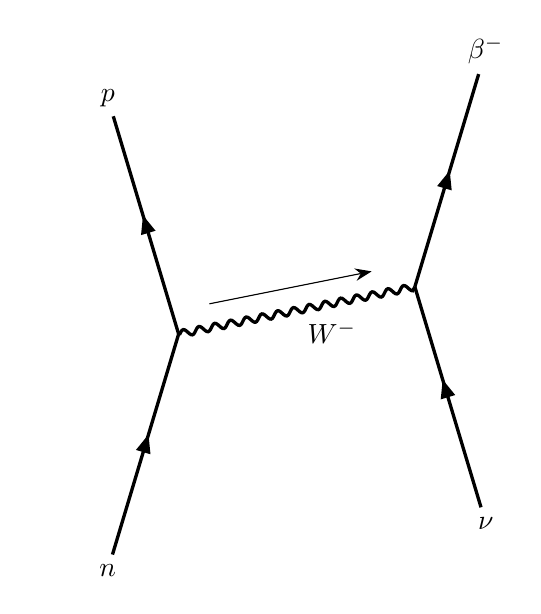
\begin{tikzpicture}[x=30mm, y=30mm]
    \begin{feynman}
        \vertex (i1) {};
        \vertex[right=.3 of i1] (i3) {\(n\)};
        \vertex[above=2 of i1] (f1) {};
        \vertex[right=.3 of f1] (f3) {\(p\)};
        \vertex[above=1 of i3] (a);
        \vertex[right=.15 of a] (b);
        \vertex[right=.15 of b] (c);
        \vertex at ($(c) + (1,.2)$) (d);
        \vertex at ($(d) + (.3, 1)$) (f4) {\(\beta^-\)};
        \vertex at ($(d) + (.3,-1)$) (f5) {\(\nu\)};
    \diagram*{
        (i3) -- [fermion, very thick] (c) -- [fermion, very thick] (f3),
        (c) -- [boson, edge label'=\(W^- \), momentum, very thick] (d),
        (d) -- [anti fermion, very thick] (f5),
        (d) -- [fermion, very thick] (f4),
    };
    % \draw[-stealth] (-.4,-.4) -- (-.4,2.2);
    % \node at (-.4,2.3) {\(t\)};
    \end{feynman}
    \end{tikzpicture}
\end{minipage}
\begin{minipage}{.45\textwidth}
  \centering
  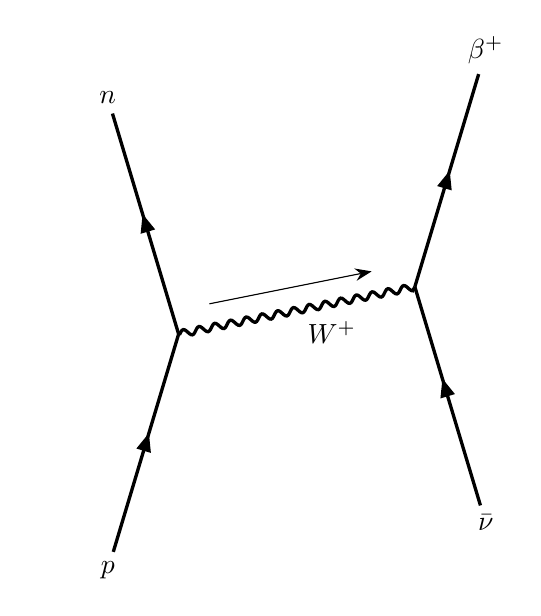
\begin{tikzpicture}[x=30mm, y=30mm]
    \begin{feynman}
        \vertex (i1) {};
        \vertex[right=.3 of i1] (i3) {\(p\)};
        \vertex[above=2 of i1] (f1) {};
        \vertex[right=.3 of f1] (f3) {\(n\)};
        \vertex[above=1 of i3] (a);
        \vertex[right=.15 of a] (b);
        \vertex[right=.15 of b] (c);
        \vertex at ($(c) + (1,.2)$) (d);
        \vertex at ($(d) + (.3, 1)$) (f4) {\(\beta^+\)};
        \vertex at ($(d) + (.3,-1)$) (f5) {\(\bar{\nu}\)};
    \diagram*{
        (i3) -- [fermion, very thick] (c) -- [fermion, very thick] (f3),
        (c) -- [boson, edge label'=\(W^+ \), momentum, very thick] (d),
        (d) -- [anti fermion, very thick] (f5),
        (d) -- [fermion, very thick] (f4),
    };
    % \draw[-stealth] (-.4,-.4) -- (-.4,2.2);
    % \node at (-.4,2.3) {\(t\)};
    \end{feynman}
    \end{tikzpicture}
\end{minipage}

\caption{The interaction between a lepton and hadron}
\end{figure}

\subsection{Photons \& Energy}
\label{sec:orgf95d016}

When charged particles undergo some change in energy, electromagnetic waves are created. These exist in \emph{discrete} packets called \emph{photons}. The energy of a photon is tied to the frequency of the wave it represents in the form:

\[E = hf\]

\subsubsection{Annihilation}
\label{sec:org533902e}

The energy gained by a particle is linked to its increase in mass via \(E = mc^2\). Given that an object at rest has mass, it has a corresponding \emph{rest energy}, equal to \(m_0c^2\). This energy is stored permanently as mass, although it is still subject to the laws of conservation of energy.

Where matter meets antimatter, specifically the correct \emph{antiparticle}, rest energy can be released in a process called \emph{annihilation}. The total rest mass of the two particles combined is converted into photon energy. Two photons are always produced to endure that the total difference in momentum is \(0\).


\begin{figure}[H]
\centering
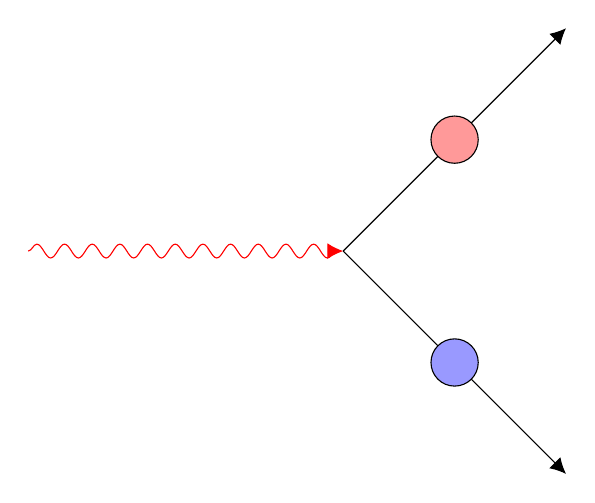
\begin{tikzpicture}
\begin{scope}[very thick,decoration={ markings, mark=at position 0.4 with {\arrow[]{Latex[length=2mm, width=2mm]}}}]
\end{scope}
\draw[draw=red, -{Latex[length=2mm, width=2mm]}, snake it] (-4,0) -- (0,0);
\draw[-{Latex[length=2mm, width=2mm]}] (0,0) -- (2.83,2.83);
\draw[-{Latex[length=2mm, width=2mm]}] (0,0) -- (2.83,-2.83);
\filldraw[fill=red!40!white, draw=black] (1.415,1.415) circle (0.3cm);
\filldraw[fill=blue!40!white, draw=black] (1.415,-1.415) circle (0.3cm);
\end{tikzpicture}
\caption{Pair production}
\end{figure}

During annihilation, the total rest mass of the particle/antiparticle pair is \(2E_0\) and two photons are produced. Therefore the minimum energy of each photon produced is equal to the rest energy of one of the particles.

\[2E_0 = 2hf_{min}\]

\[hf_{min} = E_0\]

\subsubsection{Pair Production}
\label{sec:org0f34e4c}

A high energy photon is capable of producing a particle/antiparticle pair. The energy of a photon must be equal to twice the rest mass of the particle in question, as only one photon is involved in the event.

\[hf_{min} = 2E_0\]


\begin{figure}[H]
\centering
\begin{tikzpicture}
\begin{scope}[very thick,decoration={ markings, mark=at position 0.4 with {\arrow[]{Latex[length=2mm, width=2mm]}}}]
\end{scope}
\draw[draw=red, -{Latex[length=2mm, width=2mm]}, snake it] (0,0) -- (0,4);
\draw[draw=red, -{Latex[length=2mm, width=2mm]}, snake it] (0,0) -- (0,-4);
\draw[-{Latex[length=2mm, width=2mm]}] (-4,0) -- (0,0);
\draw[-{Latex[length=2mm, width=2mm]}] (4,0) -- (0,0);
\filldraw[fill=red!40!white, draw=black] (-2,0) circle (0.3cm);
\filldraw[fill=blue!40!white, draw=black] (2,0) circle (0.3cm);
\end{tikzpicture}
\caption{Annihilation}
\end{figure}

\subsection{Quantum Phenomena}
\label{sec:org208e68e}

The word \emph{quantum} refers to a measurable, discrete quantity of something. It was theorised that energy and EM waves, along with particles, are quantised.

\subsubsection{Photoelectric Effect}
\label{sec:orgb4b892d}

The emission of electrons from the surface of a material which some electromagnetic radiation is incident on is described as the \emph{photoelectric effect}. Any electrons removed from the surface of this material are called \emph{photoelectrons}.

Traditional understanding of electromagnetism would suggest that electrons would be liberated from atoms in the material once they have absorbed enough energy from incident radiation. If this were true, photoelectrons would be emitted from a material regardless of the frequency of the incident EM wave. Greater intensity would theoretically increase the rate at which photoelectrons were emitted.

\subsubsection{Work Function \& Threshold Frequency}
\label{sec:orgc499d82}

Later evidence proved that photoelectrons were only emitted from a material when the frequency of incident radiation is greater than a certain threshold. Further increasing the frequency of incident radiation caused photoelectrons to be emitted with greater kinetic energy, indicating the presence of a constant threshold for the material. This constant was named the \emph{work function}, denoted with the symbol: \(\phi\). Therefore the final kinetic energy of an emitted photoelectron is the photon energy less the work function of the material.

\[E_{\text{Kmax}} = hf - \phi \text{ \emph{where} } E_{\text{Kmax}} > 0\]

\[f_\text{min} = \dfrac{\phi}{h}\]

Photoelectrons are only emitted from a material when \(E_{\text{Kmax}}\) exceeds \(0\). The threshold frequency, or \(f_\text{min}\), is the frequency of incident radiation required to satisfy this condition.

\subsubsection{Stopping Potential}
\label{sec:orga6c989c}

If the threshold frequency is met or exceeded, the photoelectrons that are removed from atoms can be prevented from leaving the material's surface under certain conditions. The minimum electric potential required to prevent photoelectric emission is called the \emph{stopping potential}, labelled \(V_s\). At this potential, the \(E_{\text{Kmax}}\) of each electron bearing the charge \(e\) is equal to the potential energy of the particle.

\[E_{\text{Kmax}} = eV_s\]

The electrons initial kinetic energy is reduced to 0 as work is done against the potential of the charge. Therefore the photoelectron is prevented from escaping.

\subsubsection{Vacuum Photocell}
\label{sec:org8574853}

The photoelectric effect is demonstrated in the \emph{vacuum photocell} experiment. The photocell is a glass container housing a metal plate, called the \emph{photocathode}, when \textbf{EM} radiation is incident on this plate, electrons are liberated and move the \emph{anode} on the opposite side of the photocell. The magnitude of the current in the circuit is proportional to the number of electrons reaching the anode, and hence the intensity of the light incident of the cathode.

\begin{figure}[H]
\centering
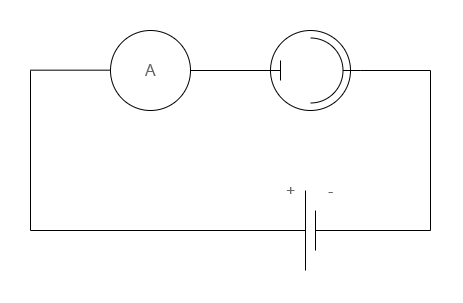
\includegraphics[width=0.7\textwidth,keepaspectratio]{./images/photoelectric_effect_circuit.png}
\caption{Vacuum photocell experiment}
\end{figure}

The \(E_{\text{Kmax}}\) of the emitted photoelectrons can be measured by raising the potential of the circuit to stopping potential, at which point the photoelectrons emitted from the photocathode do not have sufficient initial kinetic energy to overcome the potential in the photocell. As a consequence, the charge in the circuit drops to zero. The \(E_{\text{Kmax}}\) is the product of the applied potential and the magnitude of charge of an electron. Using the substitution of \(E_{\text{Kmax}} = eV_s\), the relationship formed by figure \ref{img:photoelectric_graph} is shown.

\[V_s = \dfrac{h}{e}(f - f_{min}) = \dfrac{h}{e}f - \dfrac{\phi}{e}\]

\[E_{Kmax} = hf - \phi\]

\begin{figure}[H]
\centering
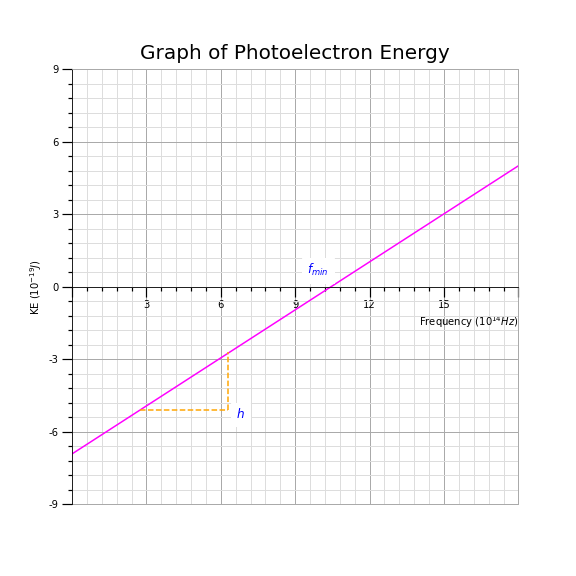
\includegraphics[width=0.9\textwidth,keepaspectratio]{./images/photoelectron_energy.png}
\caption{Kinetic energy of emitted photoelctrons}
\label{img:photoelectric_graph}
\end{figure}

\subsubsection{Ionisation}
\label{sec:orgeee2e52}

An ion is a charged atom. Positive ions are produced by removing electrons from the atom. Negative ions are produced by adding electrons to the shells around an atom. \emph{Ionisation} is the process of producing ions.

\begin{figure}[H]
\centering
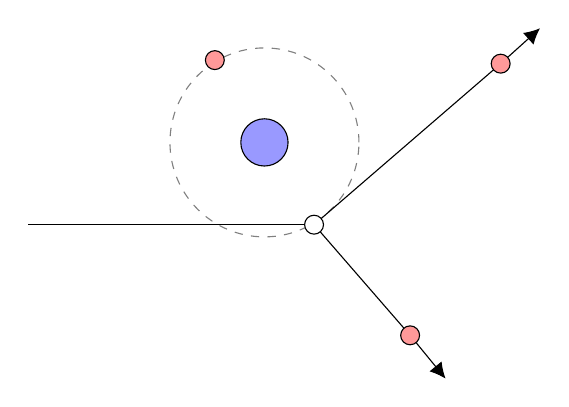
\begin{tikzpicture}
\begin{scope}[very thick,decoration={ markings, mark=at position 0.4 with {\arrow[]{Latex[length=2mm, width=2mm]}}}]
\end{scope}
\filldraw[fill=blue!40!white, draw=black] (0,0) circle (0.3cm);
\draw[dashed, gray] (0,0) circle (1.2cm);
\draw (-3,-1.045) -- (0.63,-1.045);
\draw (0.63,-1.045) -- (3,1);
\draw[-{Latex[length=2mm, width=2mm]}] (3,1) -- (3.5,1.45);
\draw (0.63,-1.045) -- (1.85,-2.45);
\draw[-{Latex[length=2mm, width=2mm]}] (1.85,-2.45) -- (2.3, -3);
\filldraw[fill=white, draw=black] (0.63,-1.045) circle (0.12cm);
\filldraw[fill=red!40!white, draw=black] (1.85,-2.45) circle (0.12cm);
\filldraw[fill=red!40!white, draw=black] (-0.63,1.045) circle (0.12cm);
\filldraw[fill=red!40!white, draw=black] (3,1) circle (0.12cm);
\end{tikzpicture}
\caption{Ionisation by collision}
\end{figure}

\subsubsection{Excitation}
\label{sec:orgbd7f80e}

During the \emph{excitation} of an electron, it is moved to a more energetic orbit, further from the atom. Unlike ionisation, electrons are not removed from the atom. Excitation may occur due to the collision of a fast moving electron with an orbitting electron, as shown on the left of figure \ref{img:electron_excitation}, or by the absorption of a photon, shown on the right of the same figure.

\begin{figure}[H]
\vspace{5mm}
\centering
\begin{minipage}{.45\textwidth}
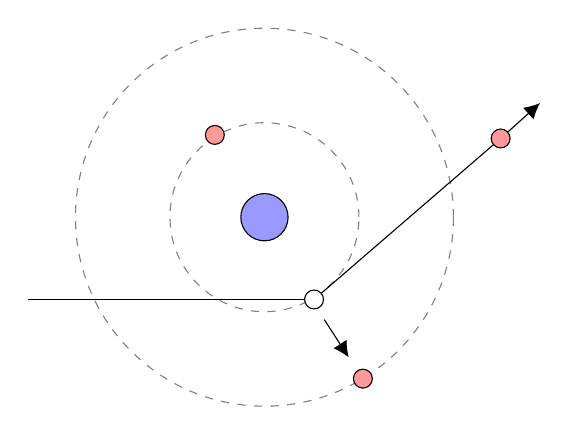
\begin{tikzpicture}
\begin{scope}[very thick,decoration={ markings, mark=at position 0.4 with {\arrow[]{Latex[length=2mm, width=2mm]}}}]
\end{scope}
\filldraw[fill=blue!40!white, draw=black] (0,0) circle (0.3cm);
\draw[dashed, gray] (0,0) circle (1.2cm);
\draw[dashed, gray] (0,0) circle (2.4cm);
\draw (-3,-1.045) -- (0.63,-1.045);
\draw (0.63,-1.045) -- (3,1);
\draw[-{Latex[length=2mm, width=2mm]}] (3,1) -- (3.5,1.45);
\draw[-{Latex[length=2mm, width=2mm]}] (0.76,-1.3) -- (1.07,-1.78);
\filldraw[fill=white, draw=black] (0.63,-1.045) circle (0.12cm);
\filldraw[fill=red!40!white, draw=black] (1.25,-2.05) circle (0.12cm);
\filldraw[fill=red!40!white, draw=black] (-0.63,1.045) circle (0.12cm);
\filldraw[fill=red!40!white, draw=black] (3,1) circle (0.12cm);
\end{tikzpicture}
\end{minipage}
\begin{minipage}{.45\textwidth}
\centering
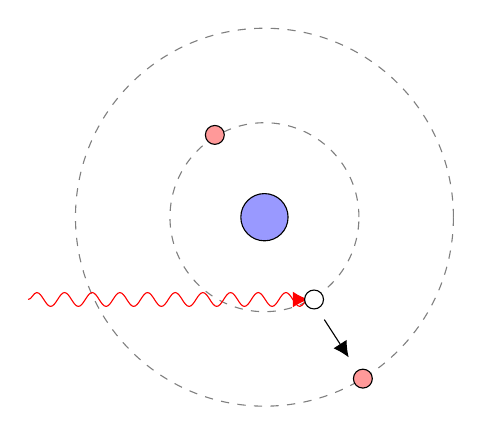
\begin{tikzpicture}
\begin{scope}[very thick,decoration={ markings, mark=at position 0.4 with {\arrow[]{Latex[length=2mm, width=2mm]}}}]
\end{scope}
\filldraw[fill=blue!40!white, draw=black] (0,0) circle (0.3cm);
\draw[dashed, gray] (0,0) circle (1.2cm);
\draw[dashed, gray] (0,0) circle (2.4cm);
\draw[draw=red, -{Latex[length=2mm, width=2mm]}, snake it] (-3,-1.045) -- (0.56,-1.045);
\draw[-{Latex[length=2mm, width=2mm]}] (0.76,-1.3) -- (1.07,-1.78);
\filldraw[fill=white, draw=black] (0.63,-1.045) circle (0.12cm);
\filldraw[fill=red!40!white, draw=black] (1.25,-2.05) circle (0.12cm);
\filldraw[fill=red!40!white, draw=black] (-0.63,1.045) circle (0.12cm);
\end{tikzpicture}
\end{minipage}
\caption{Electron excitation}
\label{img:electron_excitation}
\end{figure}

\subsubsection{Energy Levels}
\label{sec:org6275eb4}

Electrons are bound to an atom by the electrostatic force of attraction to the positively charged nucleus. Electrons may only orbit in specific positions or shells. The energy of electrons in these shells is fixed and movement between them requires exact, \emph{discrete} amounts of energy. The energy required for an electron to move between shells must be delivered or emitted in a single burst.

During excitation, an electron is moved to a higher orbit, either due to collision from another electron or the absorption of a photon. This change places the atom in a heightened \emph{energy level}. Eventually the electron will move back down to its original orbit, releasing a photon of predictable energy in a process known as \emph{de-excitation}.

\begin{figure}[H]
\vspace{5mm}
\centering
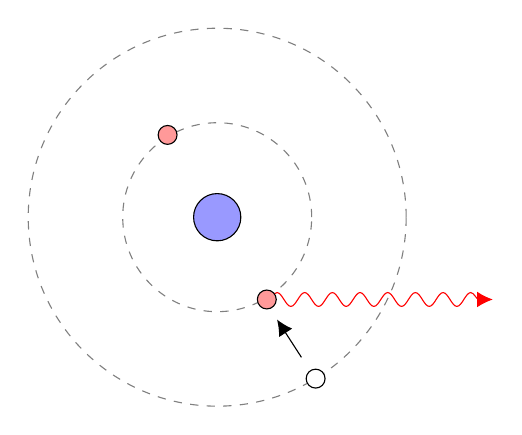
\begin{tikzpicture}
\begin{scope}[very thick,decoration={ markings, mark=at position 0.4 with {\arrow[]{Latex[length=2mm, width=2mm]}}}]
\end{scope}
\filldraw[fill=blue!40!white, draw=black] (0,0) circle (0.3cm);
\draw[dashed, gray] (0,0) circle (1.2cm);
\draw[dashed, gray] (0,0) circle (2.4cm);
\draw[draw=red, -{Latex[length=2mm, width=2mm]}, snake it] (0.65,-1.045) -- (3.5,-1.045);
\draw[-{Latex[length=2mm, width=2mm]}] (1.07,-1.78) -- (0.76,-1.3);
\filldraw[fill=red!40!white, draw=black] (0.63,-1.045) circle (0.12cm);
\filldraw[fill=white, draw=black] (1.25,-2.05) circle (0.12cm);
\filldraw[fill=red!40!white, draw=black] (-0.63,1.045) circle (0.12cm);
\end{tikzpicture}
\caption{De-excitation by emission of a photon}
\label{img:energy_levels}
\end{figure}

The diagram in figure \ref{img:energy_levels}, illustrates the \emph{energy levels} of a hypothetical atom. Each energy level, labelled on the right, is a different electronic configuration. The \emph{ionisation level} is the zero reference point and the lowest energy state of the atom is called the \emph{ground state}. As energy is \emph{required} to move the atom into a higher energy state, energy levels are negative and increase towards the ionisation level. For a change to occur, an amount of energy equal to the difference between the current energy level and any other must be absorbed or emitted.

\begin{figure}[H]
\centering
\begin{tikzpicture}
\begin{scope}[very thick,decoration={ markings, mark=at position 0.4 with {\arrow[]{Latex[length=2mm, width=2mm]}}}]
\end{scope}
\draw[thick] (-2,0) -- (2,0);
\draw[white] (-2,9) -- (2,9);
\draw[thick] (-2,8) -- (2,8);
\draw[thick] (-2,6) -- (2,6);
\draw[thick] (-2,5) -- (2,5);
\draw[very thick, red] (-2,9) -- (2,9);
\node[] at (0, 9.5) {IONISATION};
\node[] at (2.5,0) {$0$};
\node[] at (2.5,5) {$1$};
\node[] at (2.5,6) {$2$};
\node[] at (2.5,8) {$3$};
\node[] at (-2.5,0) {$-9eV$};
\node[] at (-2.5,5) {$-4eV$};
\node[] at (-2.5,6) {$-3eV$};
\node[] at (-2.5,8) {$-1eV$};
\node[] at (-2.5,9) {0};
\node[] at (-4.5, 4) {$8eV$};
\node[] at (4.5, 7) {$2eV$};
\node[] at (4.5, 5.5) {$1eV$};
\node[] at (4.5, 2.5) {$5eV$};
\draw[-{Latex[length=2mm, width=2mm]},  gray] (-1.5, 0) -- (-1.5, 8);
\draw[-{Latex[length=2mm, width=2mm]},  gray] (-0.5, 8) -- (-0.5, 6);
\draw[-{Latex[length=2mm, width=2mm]},  gray] (0.5, 6) -- (0.5, 5);
\draw[-{Latex[length=2mm, width=2mm]},  gray] (1.5, 5) -- (1.5, 0);
\draw[draw=red, -{Latex[length=2mm, width=2mm]}, snake it] (-4,4) -- (-1.5,4);
\draw[draw=red, -{Latex[length=2mm, width=2mm]}, snake it] (-0.5,7) -- (4,7);
\draw[draw=red, -{Latex[length=2mm, width=2mm]}, snake it] (0.5,5.5) -- (4,5.5);
\draw[draw=red, -{Latex[length=2mm, width=2mm]}, snake it] (1.5,2.5) -- (4,2.5);
\end{tikzpicture}
\caption{Atomic energy levels}
\label{img:energy_levels}
\end{figure}

Following excitation by a photon of \(8eV\), the atom in figure \ref{img:energy_levels}, de-excites by the emission of three less energetic photons, gradually descending through the energy levels. This phenomena is the basis of \emph{fluorescence}, where high energy \textbf{UV} photons are absorbed by fluorescent materials and the energy is released in stages as less energetic visible light photons.

\subsubsection{Wave-Particle Duality}
\label{sec:org21c4f5d}

% TODO fact check this

The diffraction of light and the photoelectric effect demonstrate light's dual particle and wave-like nature. Some particles behave the same way and have wave-like properties. The \emph{de Broglie} hypothesis states that the wave-like nature of a matter particle is characterised by its wavelength.

\[ \lambda  = \dfrac{h}{p} = \dfrac{h}{mv}\]

Evidence for the wave-like nature of matter particles comes from the diffraction of a beam of electrons. If a concentrated beam of electrons is directed through a thin metal foil, electrons are diffracted by the arrangement of positive ions. The electrons however are diffracted in particular directions.

The amount of diffraction observed can be adjusted by altering the speed of the electrons in the beam, causing a change in the \emph{de Broglie} wavelength of the beam. The beam is produced by attracting electrons from a source to a positively charged plate with a small hole in it. The speed of the electrons is therefore determined by the potential difference between these components and hence their acceleration due to the electric field in place.

Figure \ref{img:electron_diffraction} shows the diffraction of a beam of electrons through a thin metal foil, from two points of view. The image on the left, depicts a horizontal elevation of the diffraction experiment. On the right is the diffraction pattern as observed on a screen. It resembles the diffraction pattern of light directed through a single slit, rotated through \(360 \textdegree\) about its centre.

\begin{figure}[H]
\centering
\begin{minipage}{.45\textwidth}
\centering
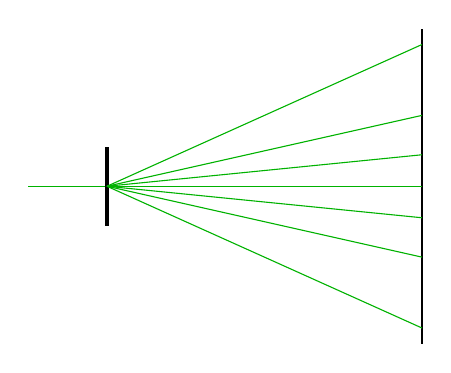
\begin{tikzpicture}
\begin{scope}[very thick,decoration={ markings, mark=at position 0.4 with {\arrow[]{Latex[length=2mm, width=2mm]}}}]
\end{scope}
\draw[green!70!black] (-3,0) -- (-2,0);
\draw[very thick] (-2,-0.5) -- (-2,0.5);
\draw[thick] (2,-2) -- (2,2);
\draw[green!70!black] (-2,0) -- (2, 0);
\draw[green!70!black] (-2,0) -- (2, 0.4);
\draw[green!70!black] (-2,0) -- (2, -0.4);
\draw[green!70!black] (-2,0) -- (2, 0.9);
\draw[green!70!black] (-2,0) -- (2, -0.9);
\draw[green!70!black] (-2,0) -- (2, 1.8);
\draw[green!70!black] (-2,0) -- (2, -1.8);
\end{tikzpicture}
\end{minipage}
\begin{minipage}{.45\textwidth}
\centering
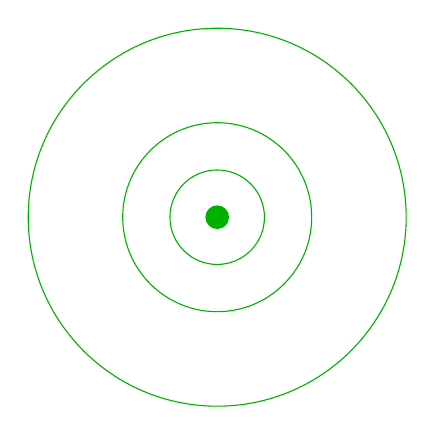
\begin{tikzpicture}
\begin{scope}[very thick,decoration={ markings, mark=at position 0.4 with {\arrow[]{Latex[length=2mm, width=2mm]}}}]
\end{scope}
\fill[green!70!black] (0,0) circle (0.15cm);
\draw[green!70!black] (0,0) circle (0.6cm);
\draw[green!70!black] (0,0) circle (1.2cm);
\draw[green!70!black] (0,0) circle (2.4cm);
\end{tikzpicture}
\end{minipage}
\caption{The diffraction of a beam of electrons}
\label{img:electron_diffraction}
\end{figure}

\section{Waves and Optics}
\label{sec:orgec17683}
\section{Mechanics}
\label{sec:org98bd5e8}
\section{Electricity}
\label{sec:orgeb8363b}
\section{Further Mechanics}
\label{sec:org5b895c6}
\section{Thermal Physics}
\label{sec:org1807a25}
\section{Fields and their Consequences}
\label{sec:org88c1261}
\subsection{Gravitational Fields}
\label{sec:orge4c8fcb}

Any object with mass creates a \emph{gravitational field} around itself. Any other mass placed within this field experiences an attractive force and exerts an equal attractive force on the first object.

\subsubsection{Gravitational Field Strength}
\label{sec:orgd002631}

If a small test mass is placed inside the gravitational field of a much larger mass, the identical force of gravitation experienced by both objects will cause a much greater acceleration to the small test mass, according to \(F = ma\). The gravitational field strength \(g\), is the force per unit mass (\(Nkg^{-1}\)) experienced by a small test mass positioned in a gravitational field. There is a direct relationship between \(g\) and the acceleration \(a\) of a small test mass.

\[g = a = \dfrac{F}{m}\]

\subsubsection{Radial and Uniform Fields}
\label{sec:org4ac81ed}

The direction of the forces surrounding a mass are shown in \emph{field-diagrams}, these represent the path taken by a small test mass in a gravitational field. The density of field lines and their proximity to one another indicate the magnitude of \(g\) at that point. The field around a planet or other spherical object is \emph{radial}. Each field line is directed towards the centre of the mass. The density of field lines decreases with distance from the mass, showing that \(g\) decreases away from a mass.

\begin{figure}[H]
\centering
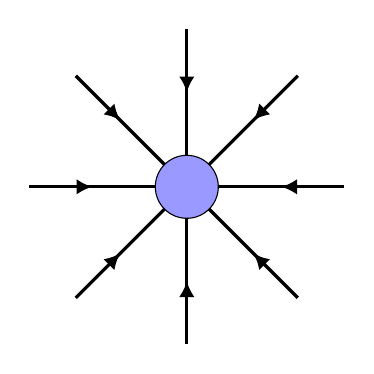
\begin{tikzpicture}
\begin{scope}[very thick,decoration={ markings, mark=at position 0.4 with {\arrow[]{Latex[length=2mm, width=2mm]}}}]
    \draw[postaction={decorate}] (0,2)--(0,0);
    \draw[postaction={decorate}] (0,-2)--(0,0);
    \draw[postaction={decorate}] (-2,0)--(0,0);
    \draw[postaction={decorate}] (2,0)--(0,0);
    \draw[postaction={decorate}] (1.41,1.41)--(0,0);
    \draw[postaction={decorate}] (1.41,-1.41)--(0,0);
    \draw[postaction={decorate}] (-1.41,1.41)--(0,0);
    \draw[postaction={decorate}] (-1.41,-1.41)--(0,0);
\end{scope}
\filldraw[fill=blue!40!white, draw=black] (0,0) circle (0.4cm);
\end{tikzpicture}
\caption{A radial graviatational field}
\end{figure}

If the same object is observed much more closely, radial field lines may appear parallel to one another and hence there is no change in the magnitude of \(g\) within the selected region of the gravitational field.

\begin{figure}[H]
\centering
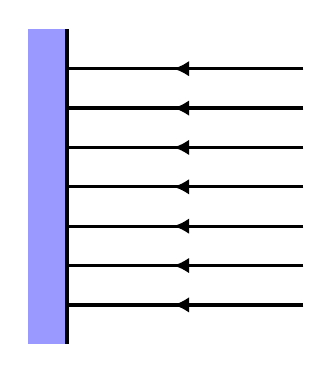
\begin{tikzpicture}
\fill[blue!40!white] (-2,2) rectangle (-1.5, -2);
\begin{scope}[very thick,decoration={ markings, mark=at position 0.55 with {\arrow[]{Latex[length=2mm, width=2mm]}}}]
    \draw[] (-1.5, 2) -- (-1.5, -2);
    \draw[postaction={decorate}]  (1.5,1.5) -- (-1.5,1.5);
    \draw[postaction={decorate}]  (1.5,1.0) -- (-1.5,1.0);
    \draw[postaction={decorate}]  (1.5,0.5) -- (-1.5,0.5);
    \draw[postaction={decorate}]  (1.5,0.0) -- (-1.5,0.0);
    \draw[postaction={decorate}]  (1.5,-0.5) -- (-1.5,-0.5);
    \draw[postaction={decorate}]  (1.5,-1.0) -- (-1.5,-1.0);
    \draw[postaction={decorate}]  (1.5,-1.5) -- (-1.5,-1.5);
\end{scope}
\end{tikzpicture}
\caption{A uniform graviatational field}
\end{figure}

\subsubsection{Gravitational Potential \& GPE}
\label{sec:org6514749}

The \emph{gravitational potential energy} is the energy of an object due to its position in a gravitational field. The \emph{gravitational potential} at a point in a gravitational field is the \emph{gravitational potential energy} per unit mass of a small test mass. It can also be described as the work done per unit mass to move an object from infinite distance to that point. Some more points:

\begin{itemize}
\item The gravitational field around an object extends to \emph{infinity}. The strength of this field diminishes with distance from the centre of the object.

\item Any object within a gravitational field will have \emph{gravitational potential energy} (the energy of an object due to its position in a gravitational field).

\item For any object in a gravitational field, its \textbf{GPE} is least when it is close to the centre of the field and larger at greater distances from the centre of the field. \textbf{GPE} is \(0\) at the infinity position. Consequently, values of \textbf{GPE} closer to the centre of the field are negative.
\end{itemize}

The unit of gravitational potential is the \(Jkg^{-1}\) and like \textbf{GPE}, values are always negative. Gravitational potential is defined as the work done per unit mass, as shown on the left. It can also be expressed in terms of \(r\) from a point mass, as is the case on the right.

\begin{figure}[H]
\centering
\begin{minipage}{.8\textwidth}
\begin{tcolorbox}[
sharp corners=all,
colback=white,
colframe=white,
size=tight,
boxrule=0.2mm,
left=10mm, right=10mm
]
\begin{multicols}{2}
\[V = \dfrac{W}{m}\]

\columnbreak

\[V = -\dfrac{GM}{r}\]
\end{multicols}
\end{tcolorbox}
\end{minipage}
\end{figure}

Therefore, at any point, the energy required to move an object from infinity to that point is:

\[\text{W} = - \dfrac{GMm}{r} \]

The work done to move a mass \(m\) a small distance \(\Delta r\) in a gravitational field can also be calculated by measuring the area under a \(g/r\) graph. More about this in section
\ref{sec:pot_grad}.

\[\Delta W = F \Delta r  = gm \Delta r \]

\[ \Delta W = \dfrac{GMm}{r^2} \Delta r \]

\subsubsection{Equipotentials}
\label{sec:org319af10}

Points in a gravitational field which are the same distance from the centre of the field will share the same value of \(V\). These loci of points are called \emph{equipotentials} and no work is done against the gravitational field when an object moves along an equipotential.

\begin{figure}[H]
\centering
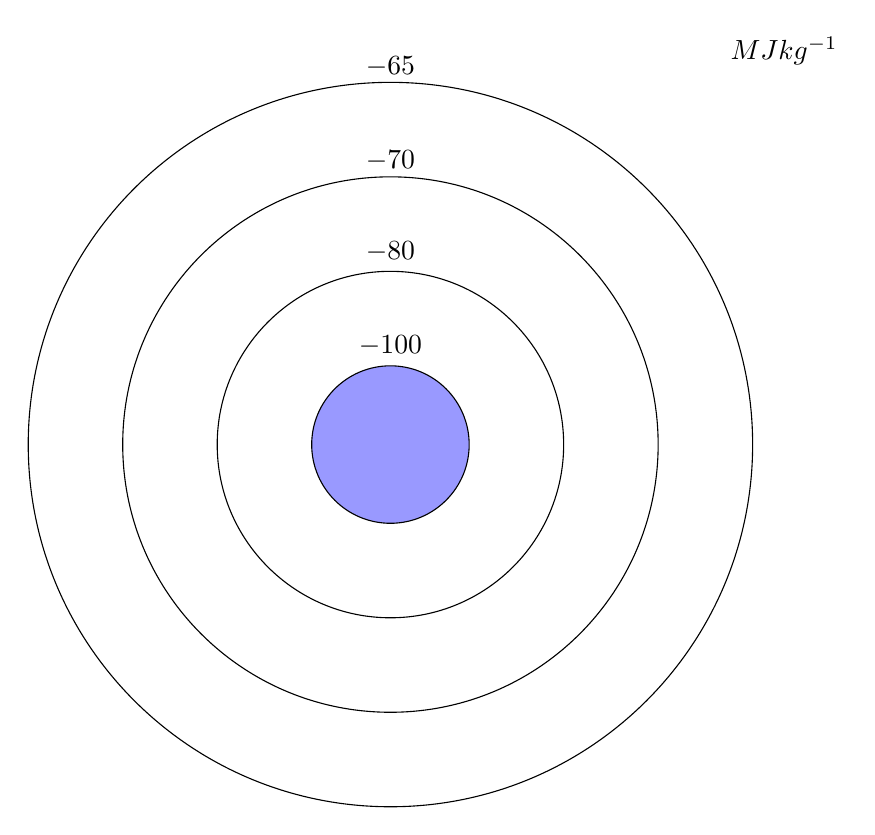
\begin{tikzpicture}
\begin{scope}[very thick,decoration={ markings, mark=at position 0.4 with {\arrow[]{Latex[length=2mm, width=2mm]}}}]
\end{scope}
\filldraw[fill=blue!40!white, draw=black] (0,0) circle (1cm);
\draw (0,0) circle (2.2cm);
\draw (0,0) circle (3.4cm);
\draw (0,0) circle (4.6cm);
\node[] at (0,1.25) {$-100$};
\node[] at (0,2.45) {$-80$};
\node[] at (0,3.6) {$-70$};
\node[] at (0,4.8) {$-65$};
\node[] at (5,5) {$MJkg^{-1}$};
\end{tikzpicture}
\caption{Equipotentials around a spherical body (not to scale)}
\end{figure}

\subsubsection{Potential Gradients}
\label{sec:org0bc89fb}
\label{sec:pot_grad}
The \emph{potential gradient} at a point in a gravitational field is the change in potential per metre at that point. As \(g\) decreases with distance from a given mass, the change in \(V\) per metre at greater distances from the centre of the field decreases. The potential gradient = \(\Delta V / \Delta r\), these values are labelled in figure \ref{img:potential_step}.

\begin{figure}[H]
\centering
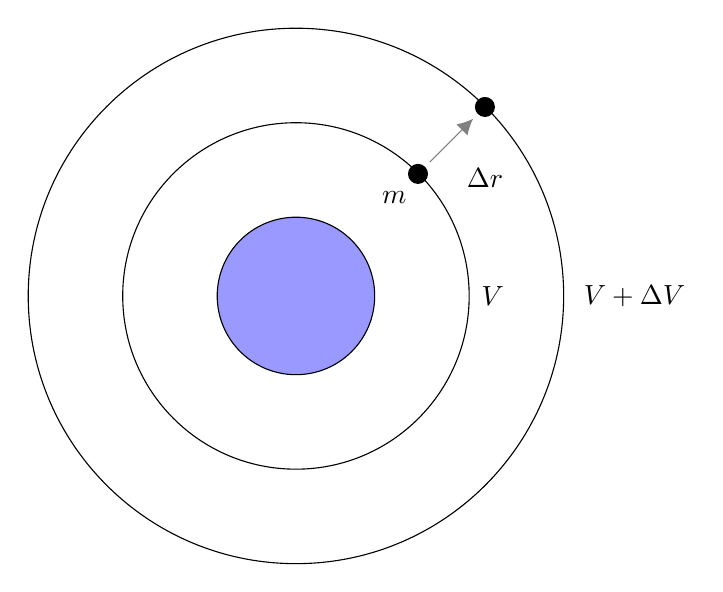
\begin{tikzpicture}
\begin{scope}[very thick,decoration={ markings, mark=at position 0.4 with {\arrow[]{Latex[length=2mm, width=2mm]}}}]
\end{scope}
\filldraw[fill=blue!40!white, draw=black] (0,0) circle (1cm);
\draw (0,0) circle (2.2cm);
\draw (0,0) circle (3.4cm);
\filldraw[black] (1.55, 1.55) circle (0.12cm);
\filldraw[black] (2.4, 2.4) circle (0.12cm);
\draw[-{Latex[length=2mm, width=2mm]}, gray] (1.7, 1.7) -- (2.25, 2.25);
\node[] at (1.25,1.25) {$m$};
\node[] at (2.5,0) {$V$};
\node[] at (4.3,0) {$V+ \Delta V$};
\node[] at (2.4,1.5) {$\Delta r$};
\end{tikzpicture}
\caption{Potential gradient}
\label{img:potential_step}
\end{figure}

If the test mass \(m\) is moved a distance \(\Delta r\) away from the planet, its \textbf{GPE} will increase as it moves to a point of higher potential. A force must be applied to the object, which is equal and opposite to the force due to gravity, acting through \(\Delta r\).

\begin{figure}[H]
\vspace{5mm}
\centering
\begin{minipage}{.8\textwidth}
\begin{tcolorbox}[
sharp corners=all,
colback=white,
colframe=white,
size=tight,
boxrule=0.2mm,
left=10mm, right=10mm
]
\begin{multicols}{2}
\noindent
\[\Delta W = F \Delta r\]

\[\Delta V = \dfrac{\Delta W}{m}\]

\[\Delta V = \dfrac{F \Delta r}{m}\]

\[F = \dfrac{m \Delta V}{\Delta r}\]

\[\textbf{\ldots}\]
% \[\scalebox{1.5}{\rotatebox[origin=c]{180}{$\Lsh$}}\]
\columnbreak
\\
\[\textbf{\ldots}\]
% \[\scalebox{1.5}{\rotatebox[origin=c]{270}{$\Rsh$}}\]

\[F_{grav} = -F\]

\[F_{grav} = - \dfrac{m \Delta V}{\Delta r}\]

\[g = \dfrac{F_{grav}}{m}\]

\[g = - \dfrac{\Delta V}{\Delta r}\]
\\

\end{multicols}
\end{tcolorbox}
\end{minipage}
\end{figure}
This proves that the gravitational field strength is the negative of the potential gradient at any point, therefore it acts in the opposite direction (towards the planet).

\subsubsection{Law of Gravitation}
\label{sec:orge89a858}

Newton's law of gravitation describes an attractive force between any two point objects. If this force is explicitly labelled an attractive force, the negative sign may be omitted. It is directly proportional to the product of the masses of the two objects and inversely proportional to the square of the separation between the two points. The constant of proportionality \(G\) is called the \emph{universal constant of gravitation}. Its value is \(6.67 \times 10^{-11} \text{} Nm^2kg^{-2}\).

\[F = \dfrac{Gm_1m_2}{r^2}\]

\subsubsection{Planetary Fields}
\label{sec:orgcc2dd96}

The field of a large spherical body such as a planet is the same as if its mass were concentrated at a single central point. For a large point mass \(M\), the force exerted on a small test mass \(m\), where \(m < M\), at distance \(r\) is determined with Newton's law of gravitation. The gravitational field strength at any point in the field is \(g = F / m\).

\begin{figure}[H]
\centering
\begin{minipage}{.8\textwidth}
\begin{tcolorbox}[
sharp corners=all,
colback=white,
colframe=white,
size=tight,
boxrule=0.2mm,
left=10mm, right=10mm
]
\begin{multicols}{2}
\[F = \dfrac{GMm}{r^2}\]

\columnbreak

\[g = \dfrac{GM}{r^2}\]
\end{multicols}
\end{tcolorbox}
\end{minipage}
\end{figure}

These equations are true if \(r > R\), where \(R\) is the radius of the planetary body; At or beyond the radius of the planet, the value of \(M\) is constant and the proportionality is accurate. The surface gravitational field strength is a special form of the equation:

\begin{figure}[H]
\centering
\begin{minipage}{.8\textwidth}
\begin{tcolorbox}[
sharp corners=all,
colback=white,
colframe=white,
size=tight,
boxrule=0.2mm,
left=10mm, right=10mm
]
\begin{multicols}{2}
\noindent
\\
\[g_s = \dfrac{GM}{R^2}\]

\[GM = R^2g_s \]

\[\textbf{\ldots}\]
% \[\scalebox{1.5}{\rotatebox[origin=c]{180}{$\Lsh$}}\]
\\
\columnbreak
\\
\[\textbf{\ldots}\]
% \[\scalebox{1.5}{\rotatebox[origin=c]{270}{$\Rsh$}}\]

\[g = \dfrac{GM}{r^2}\]

\[g = \dfrac{R^2g_s}{r^2}\]
\\

\end{multicols}
\end{tcolorbox}
\end{minipage}
\end{figure}

Values of \(r\) that are smaller than \(R\) indicate positions within the planet itself. At these positions, only the mass located in the hypothetical sphere with radius of the original centre of the planet to the current position \(r\). Within the planet, \(g\) decreases along with \(r\) to 0 at the centre, as the mass at the exact centre is 0.

\begin{figure}[H]
\centering
\begin{minipage}{.8\textwidth}
\begin{tcolorbox}[
sharp corners=all,
colback=white,
colframe=white,
size=tight,
boxrule=0.2mm,
left=10mm, right=10mm
]
\begin{multicols}{2}
\noindent

\[g = \dfrac{GM}{r^2}\]

\[V = \dfrac{4}{3} \pi r^3\]

\[M = \rho V\]

\[\textbf{\ldots}\]
\columnbreak

\[\textbf{\ldots}\]

\[M = \dfrac{4}{3} \rho \pi r^3\]

\[g = \dfrac{G \dfrac{4}{3} \rho \pi r^3}{r^2}\]

\[g = \dfrac{4}{3} G \rho \pi r\]
\end{multicols}
\end{tcolorbox}
\end{minipage}
\end{figure}

This final form of the equation is only valid when \(r < R\). This equation demonstrates a different type of relationship between \(g\) and \(r\) to the initial equation for \(g\). When \(g\) is plotted against \(r\), the relationship is linear and positive between \(0\) and \(R\). Beyond \(R\), the relationship is one of the form \(k/r^2\).

\begin{figure}[H]
\centering
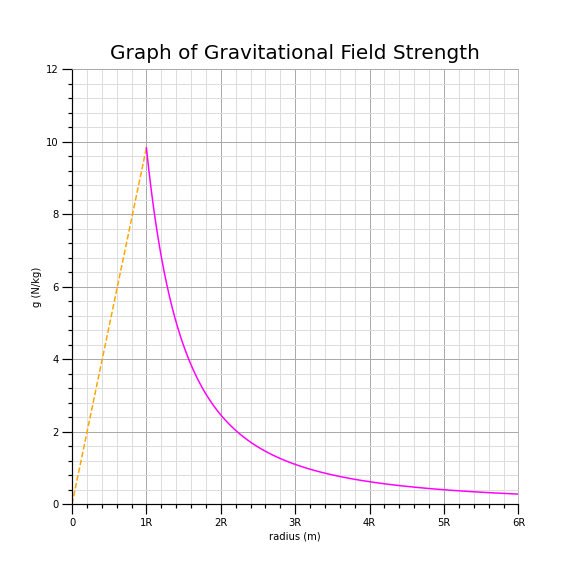
\includegraphics[width=0.9\textwidth,keepaspectratio]{./images/gravitational_field_strength.png}
\caption{Field strength within and beyond R}
\end{figure}

\subsubsection{Escape Velocity}
\label{sec:org5863e96}

If an object of mass \(m\) is positioned on the surface of a planet with mass \(M\) and radius \(R\) the \emph{escape velocity} is the velocity it must be given to escape the gravitational field of the planet. Scientifically speaking, \emph{escape velocity} is the speed at which the sum of an object's kinetic energy and its gravitational potential energy is equal to zero. A rocket propelled by its own engines can escape a field without ever reaching escape velocity, as work done by its engines will add kinetic energy. Algebraically:

\begin{figure}[H]
\centering
\begin{minipage}{.8\textwidth}
\begin{tcolorbox}[
sharp corners=all,
colback=white,
colframe=white,
size=tight,
boxrule=0.2mm,
left=10mm, right=10mm
]
\begin{multicols}{2}
\noindent

\[\dfrac{1}{2} m v^2 \ge \Delta W\]

\[\dfrac{1}{2} m v^2 \ge \dfrac{GMm}{r}\]

\[ v_{esc} = \sqrt{\dfrac{2GM}{r}}\]

\[\textbf{\ldots}\]
\columnbreak


\[\textbf{\ldots}\]

\[g = \dfrac{GM}{R^2}\]

\[ v_{esc} = \sqrt{2gR}\]
\\

\end{multicols}
\end{tcolorbox}
\end{minipage}
\end{figure}

The graph of \(V\) against \(r\) proves the \(1/r\) relationship. At any point the gradient is \(\Delta V / \Delta r\), which is equal to \(-g\).

\begin{figure}[H]
\centering
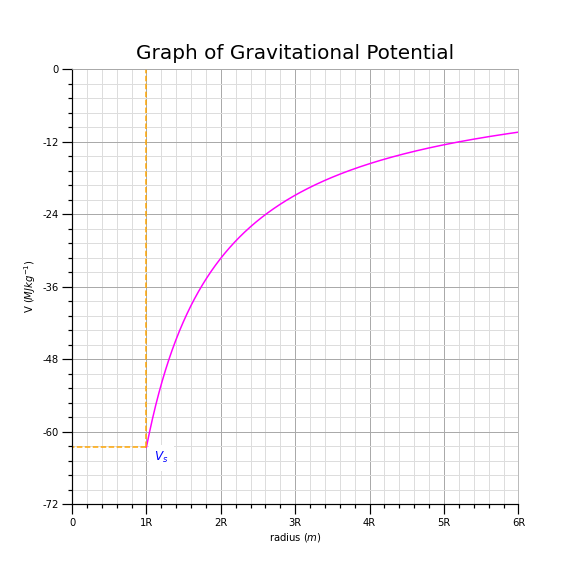
\includegraphics[width=0.9\textwidth,keepaspectratio]{./images/gravitational_potential.png}
\caption{Increase in potential with radius}
\end{figure}

\subsubsection{Satellite Motion}
\label{sec:org05dee79}

According to \emph{Kepler's Third Law}, the time period of a planet orbiting the sun depends on the mean radius of the orbit,  \(T^2 \propto r^3\). The gravitational force of attraction between a body and a satellite is the centripetal force acting on the satellite. Therefore, the gravitational field strength is equivalent to centripetal acceleration.

\begin{figure}[H]
\centering
\begin{minipage}{.8\textwidth}
\begin{tcolorbox}[
sharp corners=all,
colback=white,
colframe=white,
size=tight,
boxrule=0.2mm,
left=10mm, right=10mm,
]
\begin{multicols}{2}
\noindent
\\
\[\dfrac{v^2}{r} = \dfrac{GM}{r^2}\]

\[v^2 = \dfrac{GM}{r}\]

\[\left (\dfrac{2 \pi r}{T} \right )^2 = \dfrac{GM}{r}\]

\[\textbf{\ldots}\]
% \[\scalebox{1.5}{\rotatebox[origin=c]{180}{$\Lsh$}}\]
\columnbreak

\[\textbf{\ldots}\]

\[\dfrac{4 \pi^2 r^2}{T^2} = \dfrac{GM}{r}\]

\[\dfrac{r^3}{T^2} = \dfrac{GM}{4 \pi^2 }\]
\\

\end{multicols}
\end{tcolorbox}
\end{minipage}
\end{figure}

Seeing as \textbf{RHS} is a constant, the value of \(r^3/T^2\) is also constant for all planets. The \textbf{KE} and \textbf{PE} of an orbiting satellite are as follows:

\vspace{5mm}
\begin{figure}[H]
\centering
\begin{minipage}{.8\textwidth}
\begin{tcolorbox}[
sharp corners=all,
colback=white,
colframe=white,
size=tight,
boxrule=0.2mm,
left=10mm, right=10mm,
]
\begin{multicols}{2}
\noindent
\[v^2 = \dfrac{GM}{r}\]

\[E_k = \dfrac{1}{2} m v^2\]

\[E_k = \dfrac{GMm}{2r}\]

\[E_p = -\dfrac{GMm}{r}\]

\[\textbf{\ldots}\]
\columnbreak
\[\textbf{\ldots}\]

\[ E = E_k + E_p\]

\[E = \dfrac{GMm}{2r} -\dfrac{GMm}{r} \]

\[E =-\dfrac{GMm}{2r} \]
\\

\end{multicols}
\end{tcolorbox}
\end{minipage}
\end{figure}

\subsection{Electric Fields}
\label{sec:org4be6bf7}

Like masses, charges produce a force-field around themselves. Any two objects with like-charges create equal and opposite forces on one another. If one of these charges is a small test charge in the field of a much larger charge it will follow a path away from the body with the larger charge, along a field line.

Unlike gravitational fields, electric fields may be attractive or repulsive. Electric fields are defined in terms of positive charge and field lines indicate the direction a small positive test charge might take. Figure \ref{img:isolated_charges} shows the field lines around an isolated positive charge on the left and the equivalent field around a negative charge on the right.

\begin{figure}[H]
\centering
\begin{minipage}{.45\textwidth}
\centering
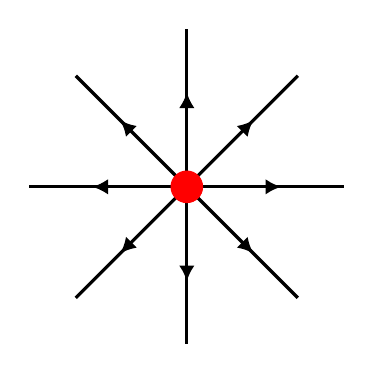
\begin{tikzpicture}
\begin{scope}[very thick,decoration={ markings, mark=at position 0.6 with {\arrow[]{Latex[length=2mm, width=2mm]}}}]
    \draw[postaction={decorate}] (0,0)--(0,2);
    \draw[postaction={decorate}] (0,0)--(0,-2);
    \draw[postaction={decorate}] (0,0)--(-2,0);
    \draw[postaction={decorate}] (0,0)--(2,0);
    \draw[postaction={decorate}] (0,0) -- (1.41,1.41);
    \draw[postaction={decorate}] (0,0) -- (1.41,-1.41);
    \draw[postaction={decorate}] (0,0) -- (-1.41,1.41);
    \draw[postaction={decorate}] (0,0) -- (-1.41,-1.41);
\end{scope}
\filldraw[red] (0,0) circle (0.2cm);
\end{tikzpicture}
\end{minipage}
\begin{minipage}{.45\textwidth}
\centering
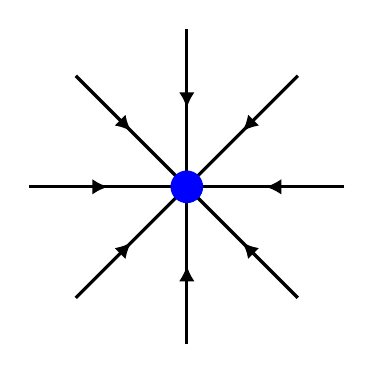
\begin{tikzpicture}
\begin{scope}[very thick,decoration={ markings, mark=at position 0.5 with {\arrow[]{Latex[length=2mm, width=2mm]}}}]
    \draw[postaction={decorate}] (0,2)--(0,0);
    \draw[postaction={decorate}] (0,-2)--(0,0);
    \draw[postaction={decorate}] (-2,0)--(0,0);
    \draw[postaction={decorate}] (2,0)--(0,0);
    \draw[postaction={decorate}] (1.41,1.41)--(0,0);
    \draw[postaction={decorate}] (1.41,-1.41)--(0,0);
    \draw[postaction={decorate}] (-1.41,1.41)--(0,0);
    \draw[postaction={decorate}] (-1.41,-1.41)--(0,0);
\end{scope}
\filldraw[blue] (0,0) circle (0.2cm);
\end{tikzpicture}
\end{minipage}
\caption{The field around isolated charges}
\label{img:isolated_charges}
\end{figure}

Placing two opposite charges near each other produces the field pattern seen in figure \ref{img:opposite_charges}. A positive charge would be repelled from the positive charge and drawn towards the negative charge.

\begin{figure}[H]
\centering
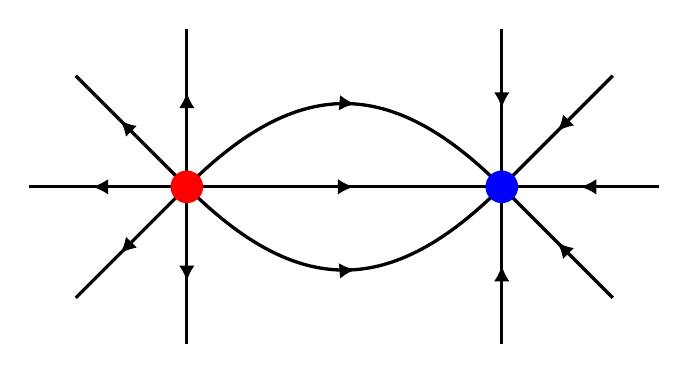
\begin{tikzpicture}
\filldraw[red] (-2, 0) circle (0.1cm);
\filldraw[blue] (2, 0) circle (0.1cm);
\begin{scope}[very thick,decoration={ markings, mark=at position 0.6 with {\arrow[]{Latex[length=2mm, width=2mm]}}}]
    \draw[postaction={decorate}] (-2,0)--(-4,0);
    \draw[postaction={decorate}] (-2,0)--(-2,2);
    \draw[postaction={decorate}] (-2,0)--(-2,-2);
    \draw[postaction={decorate}] (-2,0)--(-3.41,1.41);
    \draw[postaction={decorate}] (-2,0)--(-3.41,-1.41);
\end{scope}
\begin{scope}[very thick,decoration={ markings, mark=at position 0.5 with {\arrow[]{Latex[length=2mm, width=2mm]}}}]
    \draw[postaction={decorate}] (4,0) -- (2,0);
    \draw[postaction={decorate}] (2,2) -- (2,0);
    \draw[postaction={decorate}] (2,-2) -- (2,0);
    \draw[postaction={decorate}] (3.41,1.41) -- (2,0);
    \draw[postaction={decorate}] (3.41,-1.41) -- (2,0);
\end{scope}
\begin{scope}[very thick,decoration={ markings, mark=at position 0.53
with {\arrow[]{Latex[length=2mm, width=2mm]}}}]
    \draw[postaction={decorate}] (-2,0) -- (2,0);
    \draw[postaction={decorate}] (-2,0) .. controls (-0.59, 1.41) and (0.59, 1.41) .. (2,0);
    \draw[postaction={decorate}] (-2,0) .. controls (-0.59, -1.41) and (0.59, -1.41) .. (2,0);
\end{scope}
\filldraw[red] (-2, 0) circle (0.2cm);
\filldraw[blue] (2, 0) circle (0.2cm);
\end{tikzpicture}
\label{img:opposite_charges}
\caption{The field around two opposite charges}
\end{figure}

If two like charges are placed near each other a repulsive force is felt by each. The asymptote in the centre of figure \ref{img:like_charges} is for illustrative purposes only. Ideally, field lines would never appear to reach this line.

\begin{figure}[H]
\centering
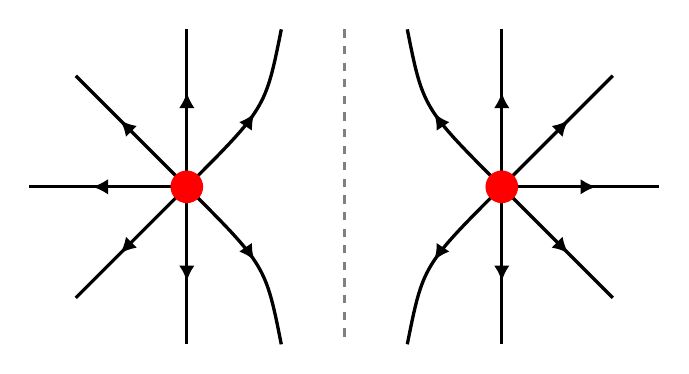
\begin{tikzpicture}
\begin{scope}[very thick,decoration={ markings, mark=at position 0.6 with {\arrow[]{Latex[length=2mm, width=2mm]}}}]
    \draw[postaction={decorate}] (-2,0)--(-4,0);
    \draw[postaction={decorate}] (-2,0)--(-2,2);
    \draw[postaction={decorate}] (-2,0)--(-2,-2);
    \draw[postaction={decorate}] (-2,0)--(-3.41,1.41);
    \draw[postaction={decorate}] (-2,0)--(-3.41,-1.41);
\end{scope}
\begin{scope}[very thick,decoration={ markings, mark=at position 0.6 with {\arrow[]{Latex[length=2mm, width=2mm]}}}]
    \draw[postaction={decorate}] (2,0)--(4,0);
    \draw[postaction={decorate}] (2,0)--(2,2);
    \draw[postaction={decorate}] (2,0)--(2,-2);
    \draw[postaction={decorate}] (2,0)--(3.41,1.41);
    \draw[postaction={decorate}] (2,0)--(3.41,-1.41);
\end{scope}
\begin{scope}[very thick,decoration={ markings, mark=at position 0.53
with {\arrow[]{Latex[length=2mm, width=2mm]}}}]
    \draw[postaction={decorate}] (-2,0) .. controls (-1, 1) .. (-0.8, 2);
    \draw[postaction={decorate}] (-2,0) .. controls (-1, -1) .. (-0.8, -2);
    \draw[postaction={decorate}] (2,0) .. controls (1, 1) .. (0.8, 2);
    \draw[postaction={decorate}] (2,0) .. controls (1, -1) .. (0.8, -2);
    \draw[gray, dashed] (0,2) -- (0, -2);
\end{scope}
\filldraw[red] (-2, 0) circle (0.2cm);
\filldraw[red] (2, 0) circle (0.2cm);
\end{tikzpicture}
\label{img:like_charges}
\caption{The field around two like charges}
\end{figure}

\subsubsection{Electric Field Strength}
\label{sec:org3eb250f}

The electric field strength \(E\) at a point in an electric field is the force per unit charge on a positive test charge placed at that point.

\[E = \dfrac{F}{Q}\]

\subsubsection{Uniform Electric Fields}
\label{sec:org15149cf}

The field lines between two parallel oppositely charged plates are parallel to one another and perpendicular to the plates. The field lines are directed from the positive to negative plate. The field lines are evenly spaced throughout the field, therefore \(E\) is the same at every point in the field. The electric field strength is given by the potential difference over the separation of the two plates.

\begin{figure}[H]
\centering
\begin{minipage}{.8\textwidth}
\begin{tcolorbox}[
sharp corners=all,
colback=white,
colframe=white,
size=tight,
boxrule=0.2mm,
left=10mm, right = 10mm,
]
\begin{multicols}{2}

\[F = QE\]

\[W = Fd = QEd\]

\[V = \dfrac{W}{Q} = \dfrac{QEd}{Q}\]

\[\textbf{\ldots}\]
\columnbreak

\[\textbf{\ldots}\]

\[V = Ed\]

\[E = \frac{V}{d}\]
\\
\\

\end{multicols}
\end{tcolorbox}
\end{minipage}
\end{figure}

\begin{figure}[H]
\centering
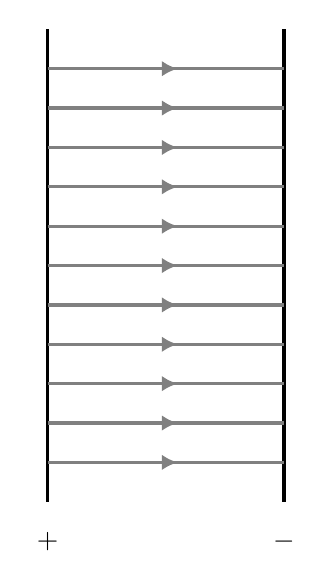
\begin{tikzpicture}
\begin{scope}[very thick,decoration={ markings, mark=at position 0.55 with {\arrow[]{Latex[length=2mm, width=2mm]}}}]
    \draw[] (-1.5, 3) -- (-1.5, -3);
    \draw[] (1.5, 3) -- (1.5, -3);
    \draw[postaction={decorate}, gray] (-1.5,2.5) -- (1.5,2.5);
    \draw[postaction={decorate}, gray] (-1.5,2.0) -- (1.5,2.0);
    \draw[postaction={decorate}, gray] (-1.5,1.5) -- (1.5,1.5);
    \draw[postaction={decorate}, gray] (-1.5,1.0) -- (1.5,1.0);
    \draw[postaction={decorate}, gray] (-1.5,0.5) -- (1.5,0.5);
    \draw[postaction={decorate}, gray] (-1.5,0.0) -- (1.5,0.0);
    \draw[postaction={decorate}, gray] (-1.5,-0.5) -- (1.5,-0.5);
    \draw[postaction={decorate}, gray] (-1.5,-1.0) -- (1.5,-1.0);
    \draw[postaction={decorate}, gray] (-1.5,-1.5) -- (1.5,-1.5);
    \draw[postaction={decorate}, gray] (-1.5,-2.0) -- (1.5,-2.0);
    \draw[postaction={decorate}, gray] (-1.5,-2.5) -- (1.5,-2.5);
\end{scope}
\node[] at (-1.5,-3.5) {$+$};
\node[] at (1.5,-3.5) {$-$};
\end{tikzpicture}
\caption{A uniform electric field}
\end{figure}

\subsubsection{Electric Potential}
\label{sec:org82dd880}

The electric potential at a point in an electric field is the energy per positive unit charge required to move it from infinity to that point. The potential gradient at a point in an electrical field is the change in potential per unit change of distance in an a given direction. The electric field strength is equal to the negative potential gradient:

\[E = - \dfrac{\Delta V}{ \Delta x}\]

\subsubsection{Coulomb's Law}
\label{sec:org4442632}

Coulomb's law links the magnitude of force existing between two point charges with the distance between them. This is an inverse square relationship. The constant of proportionality \(k\) incorporates \(\epsilon_0\), the permittivity of free space, its value is \(8.85 \times 10^{-12}\).

\begin{figure}[H]
\centering
\begin{minipage}{.8\textwidth}
\begin{tcolorbox}[
sharp corners=all,
colback=white,
colframe=white,
size=tight,
boxrule=0.2mm,
left=10mm, right=10mm
]
\begin{multicols}{2}
\[F = \dfrac{kQ_1Q_2}{r^2}\]

\columnbreak

\[k = \dfrac{1}{4 \pi \epsilon_0}\]
\end{multicols}
\end{tcolorbox}
\end{minipage}
\end{figure}

Fields are often defined in terms of a small \emph{positive} test charge \(q\) in an electric field around the more significant charge \(+Q\). If \(Q\) was a negative charge, the value of \(E\) would also be negative, indicating an attractive force on the positive test charge \(q\). The various properties of such a field are defined in the set of equations below.

\begin{figure}[H]
\vspace{5mm}
\centering
\begin{minipage}{0.8\textwidth}
\begin{tcolorbox}[
sharp corners=all,
colback=white,
colframe=white,
size=tight,
boxrule=0.2mm,
left=10mm, right=10mm,
]
\begin{multicols}{2}
\noindent
\[F = \dfrac{Qq}{4 \pi \epsilon_0r^2}\]

\[E = F/q\]

\[E = \dfrac{Q}{4 \pi \epsilon_0r^2}\]

\[\textbf{\ldots}\]
\columnbreak
\[\textbf{\ldots}\]

\[V = \dfrac{Q}{4 \pi \epsilon_0r}\]

\[E_p = \dfrac{Qq}{4 \pi \epsilon_0r}\]
\\

\end{multicols}
\end{tcolorbox}
\end{minipage}
\label{equ:e_field}
\end{figure}

\subsection{Capacitors}
\label{sec:orgd170550}

A capacitor is a component designed to store charge. Two metal plates positioned near one another form a capacitor. When connected across the terminals of a battery, electrons are forced from the negative terminal of the battery onto one of the capacitor plates. A similar number of electrons leave the opposite plate of the capacitor. Each plate gains an equal and opposite charge.

\subsubsection{Charge \& Energy Stored in a Capacitor}
\label{sec:org3e1423a}
\label{pos:constant_current_charge}

If the total charge stored on a capacitor is \(Q\), the charge on each plate is equal to \(\pm Q\). If a capacitor is charged at constant current, the \emph{capacitance} is said to be the charge stored per volt.

\[C = \dfrac{Q}{V}\]

As a capacitor is charged, the potential difference across it increases, until it is equal to the source potential difference in an ideal circuit. In order to deliver a constant charging current, a variable resistor is required to adjust the current flowing in the circuit, shown in figure \ref{img:capacitor_charge_circuit}.

\begin{figure}[H]
\centering
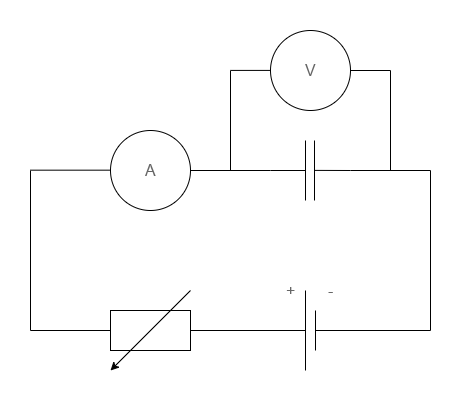
\includegraphics[width=0.7\textwidth,keepaspectratio]{./images/capacitor_charge_circuit.png}
\caption{Capacitor charging circuit}
\label{img:capacitor_charge_circuit}
\end{figure}

Assuming the current is kept constant for the duration of the charge cycle, the amount of charge on the plates after a certain time is \(Q = It\). If the potential difference is recorded at intervals of \(t\), the charge stored at that point can be calculated. When these two series are plotted against each other, the gradient is a constant equal to the capacitance \(C\), a relationship shown in figure \ref{img:capacitor_charge_constant_current_diagram}.

\begin{figure}[H]
\centering
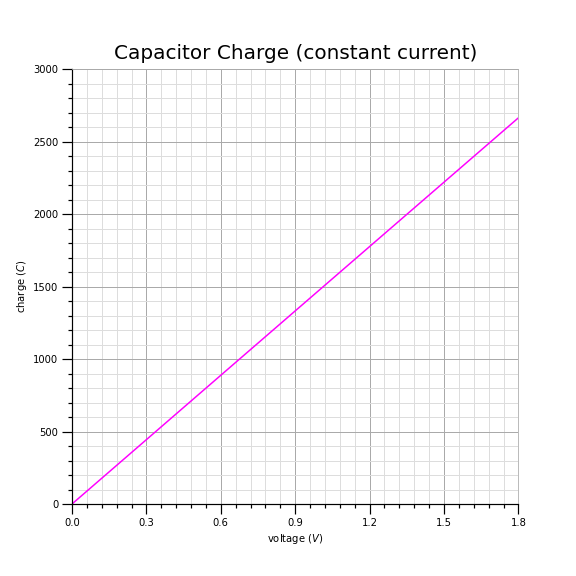
\includegraphics[width=0.9\textwidth,keepaspectratio]{./images/capacitor_charge_constant_current.png}
\caption{Charge stored in a capacitor}
\label{img:capacitor_charge_constant_current_diagram}
\end{figure}

The energy stored in a capacitor is the area under a \(V/Q\) graph.

\[E = \dfrac{1}{2} QV\]

\subsubsection{Discharging Through a Fixed Resistor}
\label{sec:orgabdc391}

If a capacitor is discharged through a fixed resistor, the discharge current decreases with time, as the charge on the plates decreases. This is a form of exponential decay, the shape of which is illustrated in figure \ref{img:capacitor_exp_discharge_graph}. The quantities current, potential difference and charge may all be used interchangeably in the equation below.

\[X = X_0 e^{-t/RC}\]

This relationship can be used to calculate a quantity \(t\) seconds after the discharge began. The value \(X_0\) is the initial quantity.

\begin{figure}[H]
\centering
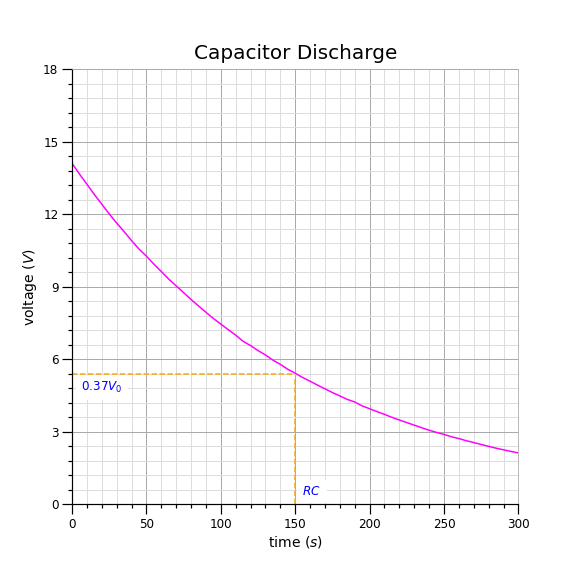
\includegraphics[width=0.9\textwidth,keepaspectratio]{./images/capacitor_exp_discharge.png}
\caption{The P.d. across a discharging capacitor}
\label{img:capacitor_exp_discharge_graph}
\end{figure}

An important quantity in the discharge or charge of a capacitor is the \emph{Time Constant}, \(\tau\). Its value is the product of \(R\), the resistance of the fixed resistor, and \(C\), the capacitance of the capacitor, according to \(\tau = RC\). When the time \(t\) equals \(\tau\), any observed quantity of the discharging capacitor arrangement will have fallen to \(e^{-1} \approx 0.37\) its initial value.

\subsubsection{Charging Through a Fixed Resistor}
\label{sec:org25c1976}

In section \(\ref{pos:constant_current_charge}\), the capacitor was charged under constant current. A variable resistor was adjusted constantly to achieve this. If a capacitor is charged through a system with \textbf{fixed} resistance, the same type of relationship seen during discharge is observed. The potential difference across the capacitor will increase to the \textbf{PD} of the circuit's source of \textbf{EMF}. The charge stored on the capacitor will increase during this time, at a rate which decreases with time. Charging current, on the other hand, will decrease gradually as the potential difference of the capacitor grows.

The charging curve for potential difference and charge are asymptotic to the initial circuit value and are the reflection of the exponential decay curve in this line. In the equations below, \(V_0\) and \(CV_0\) have been factorised from the terms on the \textbf{RHS}. The time constant is of similar significance in these relationships, where \(\tau\) is equal to the point where the charge or potential difference is \(0.63\), or \(1 - 0.37\), its final value.

\begin{figure}[H]
\centering
\begin{minipage}{0.95\textwidth}
\begin{tcolorbox}[
sharp corners=all,
colback=white,
colframe=white,
size=tight,
boxrule=0.2mm,
left=10mm, right=10mm,
]
\begin{multicols}{2}
\[V = V_0 \left ( 1 - e^{-t/RC} \right )\]

\columnbreak

\[Q = CV_0 \left ( 1 - e^{-t/RC} \right )\]
\end{multicols}
\end{tcolorbox}
\end{minipage}
\end{figure}

As the charging process takes place, the current in the circuit falls. Initially, the resistance of the capacitor is zero, so the current in the circuit is related to the resistance of the fixed resistor and the source of \textbf{EMF} alone. The charging curve for current resembles the discharging curve, it is exponential decay.

\begin{figure}[H]
\centering
\begin{minipage}{0.8\textwidth}
\begin{tcolorbox}[
sharp corners=all,
colback=white,
colframe=white,
size=tight,
boxrule=0.2mm,
left=10mm, right=10mm,
]
\begin{multicols}{2}
\noindent

\[I_0 = \dfrac{V_0}{R}\]

\columnbreak
\[I = I_0 e^{-t/RC}\]

\end{multicols}
\end{tcolorbox}
\end{minipage}
\end{figure}

\begin{figure}[H]
\centering
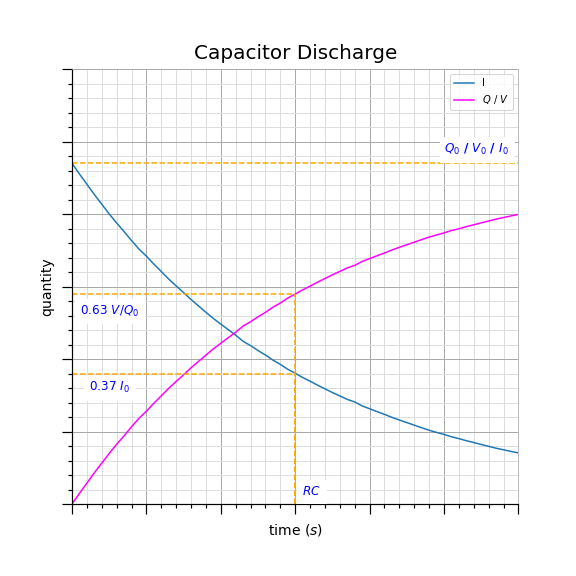
\includegraphics[width=0.9\textwidth,keepaspectratio]{./images/capacitor_exp_charge.png}
\caption{Quantities observed during capacitor charge}
\end{figure}

\subsubsection{Dielectrics}
\label{sec:org7d47ab7}

A dielectric is an insulator which is prone to polarisation when placed in an electric field. This causes the positive charges or molecules to be displaced slightly in the direction of the field and the negative charges to be moved in the opposite direction. The effect of a dielectric is to increase the charge stored between the plates of a capacitor, for a constant potential difference across its terminals. This would be an \emph{increase} in the capacitance of the capacitor.

For a capacitor at constant potential difference, more charge is stored when the plates are separated by a dielectric than a vacuum or empty space. The ratio of charge stored in the presence of a dielectric to charge stored without is know as the \emph{relative permittivity}, \(\epsilon_r\) of the dielectric material. Sometimes this quantity is know as the \emph{dielectric constant} of the material.

\begin{figure}[H]
\centering
\begin{minipage}{0.8\textwidth}
\begin{tcolorbox}[
sharp corners=all,
colback=white,
colframe=white,
size=tight,
boxrule=0.2mm,
left=10mm, right=10mm
]
\begin{multicols}{2}
\[{\epsilon}_r = \dfrac{Q}{Q_0}\]

\columnbreak

\[{\epsilon}_r = \dfrac{C}{C_0}\]
\end{multicols}
\end{tcolorbox}
\end{minipage}
\end{figure}

Relative permittivity is measured against the permittivity of free space \(\epsilon_0\). The precise permittivity of a material is the product of its dielectric constant and the permittivity of free space. For a parallel plate capacitor, its capacitance is increased by filling the space between the plates with a dielectric.

\[C = \dfrac{A {\epsilon}_r {\epsilon}_0}{d}\]

The capacitance of a capacitor is proportional to the area of one of the plates and inversely proportional to the distance between them. Inserting a dielectric material with a high relative permittivity between the plates will increase the capacitance in accordance with the expression.

\subsection{Magnetic Fields}
\label{sec:org5d5f92f}

A magnetic field surrounds any magnet or current carrying-wire, acting on another magnet or current-carrying wire. The magnetic field around a bar magnet is strongest at the poles. These poles may be \emph{north-seeking} or \emph{south-seeking}, depending on the way they align themselves with earths magnetic field. Field lines in a magnetic field illustrate the direction a north pole would move.

\subsubsection{Motor Effect}
\label{sec:orga84c904}

A wire carrying an electric current is placed at a non-zero angle to the field lines of an external magnetic field will experience a force due to its position in the field. This is known as the \emph{Motor Effect}. This force is greatest when the direction of travel of the current is perpendicular to the lines of force. The magnitude of this force will decrease to zero if the angle is reduced to zero. The magnitude of the force experienced is related to three factors: \emph{magnetic flux density}; the current in the wire and the length of wire in the field, according to:

\[F = BIL\]

This relationship demonstrates the greatest possible force given the parameters and is true when the wire is perpendicular to the field. For a piece of wire at angle \(\theta\) to the field lines, the force is:

\[F = BIL \sin (\theta )\]

Elsewhere the force may be determined in terms of \(\theta\) between the normal to the flow of current and the field lines, in which case \(\cos\) is used in place of \(\sin\).

If a single wire is placed such in a magnetic field, the force produced will move the wire out of the field. If a rectangular \emph{coil}, free to rotate in the plane parallel to the magnetic field lines, is placed in the same field, a \emph{couple} of forces are produced, which will cause rotation about this axis.

\begin{figure}[H]
\centering
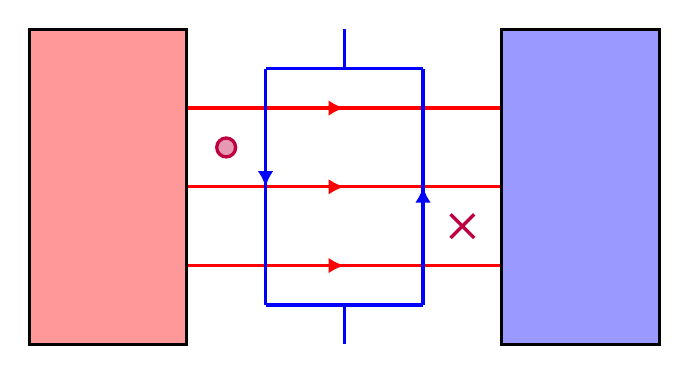
\begin{tikzpicture}
\begin{scope}[very thick,decoration={ markings, mark=at position 0.5 with {\arrow[]{Latex[length=2mm, width=2mm]}}}]
\draw[color=red, postaction={decorate}] (-2, 1) -- (2, 1);
\draw[color=red, postaction={decorate}] (-2, 0) -- (2, 0);
\draw[color=red, postaction={decorate}] (-2, -1) -- (2, -1);

\draw[color=blue, postaction={decorate}] (-1, 1.5) -- (-1, -1.5);
\draw[color=blue, postaction={decorate}] (1, -1.5) -- (1, 1.5);
\draw[color=blue] (1, -1.5) -- (-1, -1.5);
\draw[color=blue] (1, 1.5) -- (-1, 1.5);
\draw[color=blue] (0, 1.5) -- (0, 2);
\draw[color=blue] (0, -1.5) -- (0, -2);

\filldraw[fill=red!40!white, draw=black] (-2,-2) rectangle (-4, 2);
\filldraw[fill=blue!40!white, draw=black] (2,2) rectangle (4, -2);

\filldraw[fill=purple!40!white, draw=purple] (-1.5,0.5) circle (0.12cm);
\draw[purple] (1.35,-0.35) -- (1.65,-0.65);
\draw[purple] (1.35,-0.65) -- (1.65, -0.35);
\end{scope}
\end{tikzpicture}
\caption{Current-carrying coil in a magnetic field}
\label{diag:motor_side_view}
\end{figure}

The side profile of an electric motor in figure \ref{diag:motor_side_view} demonstrates the couple of forces produced when this arrangement is placed in a magnetic field. This diagram, when viewed from above, shows the angle created between the plain of the coil and the field, labelled \(\alpha\).

\begin{figure}[H]
\centering
\begin{minipage}{.45\textwidth}
\centering
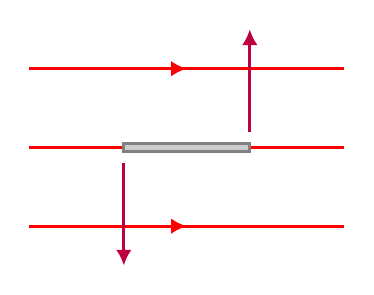
\begin{tikzpicture}
\begin{scope}[very thick,decoration={ markings, mark=at position 0.5 with {\arrow[]{Latex[length=2mm, width=2mm]}}}]
\draw[color=red, postaction={decorate}] (-2, 1) -- (2, 1);
\draw[color=red] (-2, 0) -- (2, 0);
\draw[color=red, postaction={decorate}] (-2, -1) -- (2, -1);
\filldraw[fill=gray!40!white, draw=gray] (-0.8, -0.05) rectangle (0.8, 0.05);
\draw[-{Latex[length=2mm, width=2mm]}, purple] (0.8, 0.2) -- (0.8, 1.5);
\draw[-{Latex[length=2mm, width=2mm]}, purple] (-0.8, -0.2) -- (-0.8, -1.5);
\end{scope}
\end{tikzpicture}
\end{minipage}
\begin{minipage}{.45\textwidth}
\centering
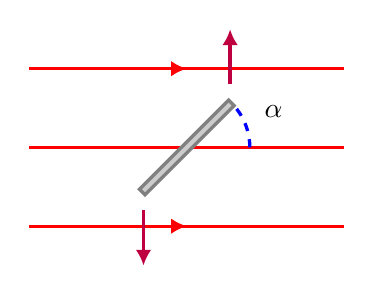
\begin{tikzpicture}
\begin{scope}[very thick,decoration={ markings, mark=at position 0.5 with {\arrow[]{Latex[length=2mm, width=2mm]}}}]
\draw[color=red, postaction={decorate}] (-2, 1) -- (2, 1);
\draw[color=red] (-2, 0) -- (2, 0);
\draw[color=red, postaction={decorate}] (-2, -1) -- (2, -1);
\draw[dashed, blue] (0.8,0) arc (0:45:0.8);
\node at (1.1,0.45) {\(\alpha\)};
\filldraw[fill=gray!40!white, draw=gray, rotate around={45:(0,0)}] (-0.8, -0.05) rectangle (0.8, 0.05);
\draw[-{Latex[length=2mm, width=2mm]}, purple] (0.55, 0.8) -- (0.55, 1.5);
\draw[-{Latex[length=2mm, width=2mm]}, purple] (-0.55, -0.8) -- (-0.55, -1.5);
\end{scope}
\end{tikzpicture}
\end{minipage}
\caption{Current-carrying coil in a magnetic field (above)}
\end{figure}

At any point during the rotation, the torque of the couple is given by the expression \(BIAn \cos (\alpha )\), where \(A\) is the area of the coil and \(\alpha\) is the angle between the plain of the coil and the field.

\subsubsection{Charges in Magnetic Fields}
\label{sec:org9d4616c}

Magnetic fields influence the passage of charged particles. A current-carrying wire experiences a force, as the paths of electrons in it are changed. Confined to the wire the  electrons cause the whole wire to experience a force.

The force on a moving charged particle is comparable to that experienced by a current-carrying wire. The passage of a current \(Q\) at speed \(v\) through a field in time \(t\) is equivalent to a current of \(Q/t\) over a length of \(vt\). The force on a particle travelling at an angle \(\theta\) to the field can also be calculated.


\begin{figure}[H]
\centering
\begin{minipage}{0.8\textwidth}
\begin{tcolorbox}[
sharp corners=all,
colback=white,
colframe=white,
size=tight,
boxrule=0.2mm,
left=10mm, right=10mm,
]
\begin{multicols}{2}
\noindent
\[F = BQv\]
\columnbreak
\[F = BQv \sin (\theta )\]
\end{multicols}
\end{tcolorbox}
\end{minipage}
\end{figure}

\subsubsection{Flux and Flux Linkage}
\label{sec:org0c9a8ad}

The magnetic flux of a field is the product of flux density, \(B\), and the given perpendicular area. Magnetic flux linkage is the product of magnetic flux and the number of turns in a coil. The unit of magnetic flux is the \textbf{weber} \((Wb)\).

\begin{figure}[H]
\centering
\begin{minipage}{0.8\textwidth}
\begin{tcolorbox}[
sharp corners=all,
colback=white,
colframe=white,
size=tight,
boxrule=0.2mm,
left=10mm, right=10mm,
]
\begin{multicols}{2}
\noindent
\[\phi = BA\]
\columnbreak
\[ N \phi = BAN\]
\end{multicols}
\end{tcolorbox}
\end{minipage}
\end{figure}

\subsubsection{Electromagnetic induction}
\label{sec:org13e9975}

Moving a wire, which is part of a circuit, through a magnetic field causes a small current to pass through the circuit. This is due to the electormotive force experienced by the wire, a consequence of electromagnetic induction. The effect occurs when a wire crosses the field lines of a magnetic field. Electromagnetic induction was discovered by Michael Farady in 1831 at the Royal Institution, London. A magnetic compass was proven to deflect from a wire when it is placed in a magnetic field. The induced voltage was labelled \emph{electromotive force}.

When a charged particle is moving through a magnetic field it feels a force, and hence an acceleration in the direction perpendicular to both the magnetic field and its motion. If a wire is moved in the same way (sweeping across magnetic field lines), electrons in the wire move along the wire, creating an \textbf{EMF} in the wire. If the wire forms part of a complete circuit, current flows as a consequence of the \textbf{EMF}.

There are two laws which govern electromagnetic induction: \emph{Lenz's law} and \emph{Faraday's law}. The former is very simple: the direction of the induced current in a circuit opposes the motion which causes it. This is a consequence of conservation of energy, it is impossible that motion in one direction could create a current which would create a force in the same direction. Faraday's law states that the magnitude of the induced \textbf{EMF} is equal to the rate of change of flux linkage. Combining the two laws, the magnitude and direction of the \textbf{EMF} can be calculated. The minus sign in the equation below indicates that the \textbf{EMF} opposes the motion that induced it, according to Lenz's law.

\[\epsilon =  - N \dfrac{\Delta \phi}{\Delta t}\]

The diagrams in figure \ref{diag:induction} illustrate electromagnetic induction. In the first (left) case, a charged particle moving to the right will experience a downward force. In the second example the charges are confined to a wire. Electrons will move downward and so conventional current flows upwards as the conductor is moved to the right. In either case, the magnetic field acts into the page.

\begin{figure}[H]
\centering
\begin{minipage}{.45\textwidth}
\centering
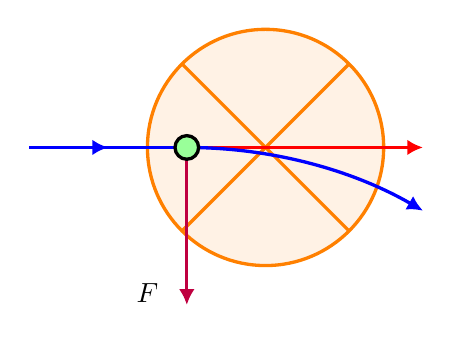
\begin{tikzpicture}
\begin{scope}[very thick,decoration={ markings, mark=at position 0.5 with {\arrow[]{Latex[length=2mm, width=2mm]}}}]
\filldraw[fill=orange!10!white, draw=orange] (0,0) circle (1.5cm);
\draw[orange, rotate around={45:(0,0)}] (-1.5, 0) -- (1.5, 0);
\draw[orange, rotate around={45:(0,0)}] (0, 1.5) -- (0, -1.5);
\draw[color=blue, postaction={decorate}] (-3, 0) -- (-1, 0);
\draw[color=red, -{Latex[length=2mm, width=2mm]}] (-1, 0) -- (2, 0);
\draw[color=purple, -{Latex[length=2mm, width=2mm]}] (-1, 0) -- (-1, -2);
\node at (-1.5,-1.85) {\(F\)};
\draw[color=blue, rotate around={-90:(-1,0)}, -{Latex[length=2mm, width=2mm]}] (-1,0) arc (0:-30:-6);
\filldraw[fill=green!40!white, draw=black] (-1,0) circle (0.15cm);
\end{scope}
\end{tikzpicture}
\end{minipage}
\begin{minipage}{.45\textwidth}
\centering
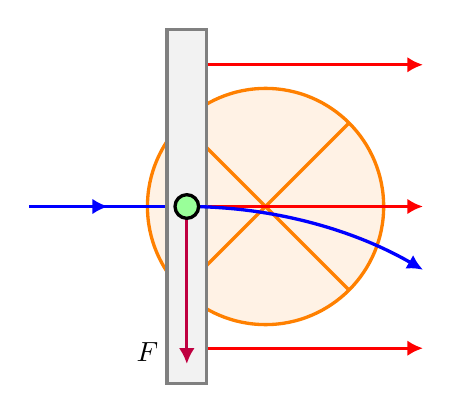
\begin{tikzpicture}
\begin{scope}[very thick,decoration={ markings, mark=at position 0.5 with {\arrow[]{Latex[length=2mm, width=2mm]}}}]
\filldraw[fill=orange!10!white, draw=orange] (0,0) circle (1.5cm);
\draw[orange, rotate around={45:(0,0)}] (-1.5, 0) -- (1.5, 0);
\draw[orange, rotate around={45:(0,0)}] (0, 1.5) -- (0, -1.5);
\draw[color=blue, postaction={decorate}] (-3, 0) -- (-1, 0);
\draw[color=red, -{Latex[length=2mm, width=2mm]}] (-1, 0) -- (2, 0);
\draw[color=red, -{Latex[length=2mm, width=2mm]}] (-1, 1.8) -- (2, 1.8);
\draw[color=red, -{Latex[length=2mm, width=2mm]}] (-1, -1.8) -- (2, -1.8);
\filldraw[fill=gray!10!white, draw=gray] (-1.25, -2.25) rectangle (-0.75, 2.25);
\draw[color=purple, -{Latex[length=2mm, width=2mm]}] (-1, 0) -- (-1, -2);
\node at (-1.5,-1.85) {\(F\)};
\draw[color=blue, rotate around={-90:(-1,0)}, -{Latex[length=2mm, width=2mm]}] (-1,0) arc (0:-30:-6);
\filldraw[fill=green!40!white, draw=black] (-1,0) circle (0.15cm);
\end{scope}
\end{tikzpicture}
\end{minipage}
\label{diag:induction}
\caption{Electromagnetic Induction}
\end{figure}

There are numerous specific examples of electromagnetic induction. For the most part, it is simply applying \(BA/\Delta t\) to calculate the \textbf{EMF}. For example the \textbf{EMF} due to a conductor (wire) moving through a field is \(Bl \Delta s / \Delta t\), which can be simplified to \(Blv\). For a rectangular coil with \(N\) turns undergoing the same motion, its EMF is \(BNlv\). For a fixed coil in a changing magnetic field, the induced force is \(AN \Delta B/ \Delta t\).

When a coil rotates at a constant frequency in a magnetic field, the emf induced can be calculated using a formula derived by finding the derivative of the formula for magnetic flux linkage with respect to time, as induced emf is equal to the rate of change of flux linkage. In this case \(\theta\), the angle between the normal to the plain of the coil and the direction of the field, is equal to \(2 \pi f t\) or \(\omega t\), where \(t\) is the number of secnods since \(\theta = 0\). The various equation involved are given below.

\begin{figure}[H]
\centering
\begin{minipage}{0.8\textwidth}
\begin{tcolorbox}[
sharp corners=all,
colback=white,
colframe=white,
size=tight,
boxrule=0.2mm,
left=10mm, right=10mm,
]
\begin{multicols}{2}
\noindent
\[N \phi = BAN \cos (\omega t) \]
\[ \epsilon = BAN \omega \sin (\omega t) \]
\columnbreak
\[\epsilon _0 = BAN \omega\]

\[ \epsilon = \epsilon _0 \sin (\omega t) \]
\\

\end{multicols}
\end{tcolorbox}
\end{minipage}
\end{figure}

\subsubsection{Solenoids and Coils}
\label{sec:org2cf18aa}

When current is passed through a coil arrangement, a magnetic field is produced. This can be verified with a plotting compass. For a large coil or \emph{solenoid} arrangement, this field resembles the field seen around a bar magnet. For illustrative purposes, current appears to flow \textbf{anticlockwise around the ``north pole'' of the solenoid} when viewed from outside.

\subsubsection{Alternating Current}
\label{sec:org23eb0f2}

Induced \textbf{EMF} is alternating, so it changes in direction periodically. As seen above \textbf{EMF} is modelled with a \(\sin\) function, therefore the graph of \textbf{EMF} against time is a sinusoidal curve. In a single cycle, the current or \textbf{EMF} is seen to move one way and then the other. The frequency of an alternating current is the number of these cycles per second.

When displayed on an oscilloscope, various measurements of an alternating current \textbf{EMF} can be measured. The \emph{peak voltage} is the displacement from equilibrium to the highest or lowest measured voltage, labelled \(V_0\). The \emph{peak-to-peak} voltage is effectively double \(V_0\), the difference between the highest measured voltage and the corresponding minimum.

The \emph{root mean square} voltage is the average of the squares of all possible voltages. This can be calculated from \(V_0\). The root mean square current is also measured in the same way.

\begin{figure}[H]
\centering
\begin{minipage}{0.8\textwidth}
\begin{tcolorbox}[
sharp corners=all,
colback=white,
colframe=white,
size=tight,
boxrule=0.2mm,
left=10mm, right=10mm,
]
\begin{multicols}{2}
\noindent
\[V_{rms} = \dfrac{V_0}{\sqrt{2}}\]
\columnbreak
\[I_{rms} = \dfrac{I_0}{\sqrt{2}}\]
\end{multicols}
\end{tcolorbox}
\end{minipage}
\end{figure}

The power lost in a conductor carrying a direct current is equal to \(I^2V\). For an alternating current the power radiated from a conductor varies with time, shown by figure \ref{img:ac_power}. At peak current the power radiated is \({I_0}^2R\), while the power is 0 when the current is 0. Due to the sinusoidal nature of the current, the average power is half of the peak power, or \(0.5 {I_0}^2 R\). This can also be written \((I_{rms})^2R\). Generally speaking, the root mean square value of an alternating current or potential difference is \(1/\sqrt{2}\) the peak value.

\begin{figure}[H]
\centering
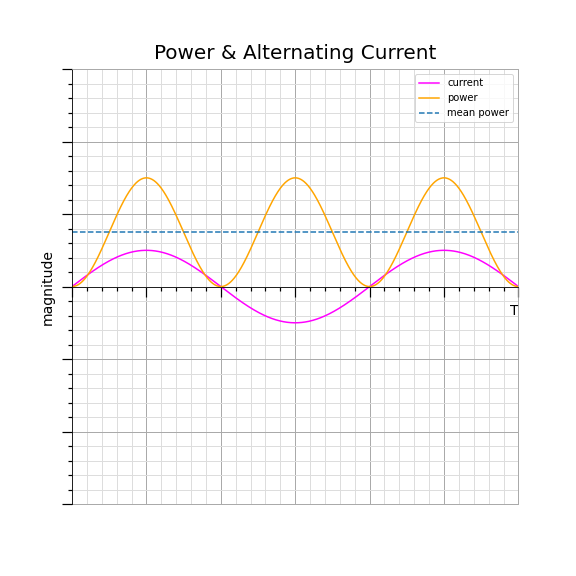
\includegraphics[width=0.9\textwidth,keepaspectratio]{./images/ac_power.png}
\caption{Power and AC quantities}
\label{img:ac_power}
\end{figure}

\subsubsection{Transformers}
\label{sec:orgeacf7e7}

A transformer is a device which is able to change the peak voltage of an alternating current. The device has two coils surrounding an ferrous iron core. The first or \emph{primary} coil is connected to the input voltage. The changing current in the wire causes an alternating magnetic field in the core. An \textbf{EMF} is induced in the secondary coil, due to the changing magnetic flux, according to \(\epsilon = AN \Delta B/\Delta t\).

\[\dfrac{N_s}{N_p} = \dfrac{V_s}{V_p}\]

\begin{figure}[H]
\centering
\begin{tikzpicture}[global scale/.style={scale=1.0}, rotate=-5, xslant=-0.1, thick, every
    node/.style={transform shape, scale=0.8}, decoration={markings, mark=at position 0.5 with {\arrow{latex}}}]
\begin{scope}[even odd rule]
\filldraw[rounded corners=2pt, fill=gray, rotate=-0, opacity=1.0] (\dx,
\dy) rectangle ++(5,5) (\lx+\dx,\ly+\dy) rectangle ++(\a, \a);
\fill [rounded corners=2pt, fill=gray] (\b, 0) --++ (0, \dy+\dr+0.02) --++(\dx, 0) --cycle;
\fill [rounded corners=2pt, fill=gray] (0, \b) --++ (\dx+\dr+0.02, 0) --++(0, \dy)--cycle;
\filldraw[rounded corners=2pt, fill=gray!50, rotate=-0] (0,0) rectangle
++(\b, \b) (\lx,\ly) rectangle ++(\a, \a);
\draw (\b-\dr,\dr) --++(\dx, \dy);
\draw (\b-\dr,\b-\dr) --++(\dx, \dy);
\draw (\dr,\b-\dr) --++(\dx, \dy);
\draw [blue, thick, postaction={decorate}] (0, \ly) --++(-1.5,0);
\foreach \z in {0,.24,.48,...,2.5}
    {
    \draw [rounded corners=2pt,blue, thick]
    (-0.0,\ly+\z+0.08)--(-0.09,\ly+\z) -- (\lx, \ly+\z)--++(0.89,0.5)
    --++(-0.08, 0.05);
}
\draw [rounded corners=2pt,blue, thick, postaction={decorate}] (-1.5,
\ly+2.8) --++(1.5,0) node[black, above, pos=0.4] {$I_p$};
\draw[latex-latex] (-\lx, \ly) --++(0, 2.8) node[midway, left] {$V_p$};

\draw [rounded corners=2pt,red, thick] (\a+\lx-2*\dr,
\ly+2*\dr)--++(-\dr, -\dr)--++(\lx+\dx+2*\dr, 0);
\draw [red, postaction={decorate}] (\b+\dx-\dr, \ly+\dr)--++(\a/2, 0);
\draw [rounded corners=2pt, red, thick, postaction={decorate}]
(\a+3*\lx-0.2, \ly+3.1) --++(\a/2, 0) node[black, midway, above] {$I_s$};
\foreach \z in {.125,.25,.375,...,2.5}
    {
    \draw [rounded corners=2pt, red, thick] (\a+\lx,\ly+\z+0.1)--
    (\a+\lx-0.07,\ly+\z) -- (\a+2*\lx, \ly+\z)--++(0.87,0.5)--++(-0.06,
    0.06);
    }
\draw[latex-latex] (2*\a+\lx, \ly) --++(0, 3.1) node[midway, left] {$V_s$};
\end{scope}
\end{tikzpicture}
\caption{An AC transformer}
\label{img:ac_transformer}
\end{figure}

Energy may be lost in a transformer due to any one of a number of reasons. The efficiency of a transformer can be calculated as follows:

\[ \text{efficiency} = \dfrac{I_sV_s}{I_pV_p}\]

Energy may be lost due to \emph{eddy currents}, induced by the alternating current of the primary core. The direction of current is so as to oppose the field due to the primary coil, which reduces the magnetic flux in the core. Eddy currents produce heat, which wastes energy. The amplitude of eddy currents are reduced by using either a high-resistivity metal for the core, a laminated core, consisting of layers of conductor separated by insulating material.

The heating effect in the coils may cause energy to be lost. This is mitigated by the use of thicker wires in the coils. Soft iron cores are preferred as they promote easy magnetisation and demagnetisation, improving the efficiency of the transformer.

\subsubsection{The Grid System}
\label{sec:org58a2218}

In the United Kingdom, electricity is generated at 50Hz, 25kV. For long distance transmission the voltage is increased to 275kV or 400kV by step-up transformers. These high voltages are stepped down in stages, first to 132kV and then to 33kV which is supplied to heavy industry. Light industry receives electricity at 11kV and homes receive electricity at 230V. The frequency of generated electricity remains at 50Hz, regardless of the voltage.
\section{Nuclear Physics}
\label{sec:org5dbe7b3}
\subsection{Radiation}
\label{sec:orgb8e3589}

Atoms which are not considered stable emit \emph{radiation}. Radiation is the emission of energy and is often \emph{electromagnetic} or as particles. Radiation is sometimes considered frightening or alarming among the general population, although it has many industrial and medical uses.

\subsection{Inverse Square Law}
\label{sec:orgd51ff71}

The intensity \(I\) of \(\gamma\) radiation is the energy transferred per second per unit area. Assuming a point source emits \(n\) \(\gamma\) photons per second and each photon has the energy \(hf\), the total energy emitted by the source per second is \(nhf\). These photons are free to leave the source in any direction, so at distance \(r\) from the source all the photons will pass through an area equal to the \emph{S.A.} of a sphere with radius \(r\). This equation represents the intensity of radiation from a point source at distance \(r\):

\[I = \dfrac{nhf}{4 \pi r^2}\]

\subsection{Hazards of Radiation}
\label{sec:org2571290}

Ionising radiation is damaging to living cells. It may cause cells to die, mutate or grow uncontrollably. The consequences may be felt by the affected individual, which is described as \emph{somatic effects}, or passed onto future generations \emph{genetically}.

To best mitigate the risks of radiation, sources should be kept in \emph{lead-lined} containers to reduce any \(\gamma\) emission from the source to background level. These sources may be kept in a secure, locked-away location and exposure / use of the source should be recorded.

During use, solid sources should be handled with handling tools, to keep the source at a distance from the body. This reduces the intensity of \(\gamma\) radiation incident on the handler and would ideally put their body beyond the range of \(\alpha\) or \(\beta\) particles. Liquid, gaseous and powdered sources should be kept in sealed containers, so they are not accidentally inhaled, ingested or split.

\subsection{Radioactive Decay}
\label{sec:org7281261}

If a radioactive isotope of element \(X\) undergoes \(\alpha\) or \(\beta\) emission, it is no longer a nucleus of the same element, due to the change in proton number. If this nucleus was one of many in a sample of a particular isotope, the number of nuclei of this isotope will decrease as individual nuclei decay. The same relationship is true of the mass of the original isotope; the mass will decrease as nuclei decay. There are three important quantities surrounding radioactive decay:

\begin{itemize}
\item The \emph{half-life} \(T_{1/2}\) of a radioactive isotope is the time take for the mass (or any other specific property) to decrease to half the initial value.

\item The \emph{activity} \(A\) of a radioactive isotope is the number of nuclei disintegrating per second, corresponds to the rate of changes of nuclei of the initial isotope. The unit of activity is the \emph{Becquerel} (Bq), where 1Bq is one disintegration per second.

\item The \emph{decay constant} \(\lambda\) is the probability of an individual nucleus decaying per unit time (usually one second).
\end{itemize}

The decay of a single nucleus is impossible to predict. Every nucleus of an isotope in a sample has an equal probability of decaying in a given interval. For a large sample of a radioactive isotope \(X\), the number of nuclei which disintegrate \(\Delta N\) in a given time period \(\Delta t\) is related to the initial number of nuclei \(N_0\), via the decay constant.

\subsubsection{Decay Constant}
\label{sec:org0fb2a65}

The probability of a single decay is the fraction of the initial number of nuclei of \(X\) which decay per second. This is called the \emph{decay constant}, and is represented with the symbol \(\lambda\). If reference is made to \emph{decay} or its decreasing nature, there is no need to include a minus sign.

\[\lambda = \dfrac{\Delta N}{N_0}/\Delta t\]

The change in number of nuclei for a combination of the given factors can be obtained by rearranging the equation above. Note the presence of the minus sign here indicating decrease.

\[ \Delta N = - \lambda N_0 \Delta t\]

\subsubsection{Activity}
\label{sec:orgfa0c2ed}

The activity of the isotope is the number of nuclei which disintegrate per second and it is proportional to the value of \(N_0\). An expression for \(A\) can be obtained as follows:

\[ \dfrac{\Delta N}{\Delta t} = - \lambda N_0\]

\[ A = - \lambda N_0\]

Therefore the activity of \(N\) nuclei of a particular isotope can also be written simply:

\[ A = \lambda N\]

\subsubsection{Decay Curves}
\label{sec:org26e6462}

As the activity, or rate of change of nuclei of \(X\), is proportional to the current number of nuclei \(N\) of \(X\), the relationship between \(t\) and \(N\) is one of exponential decay. The number of nuclei remaining after a particular time period is proportional to \(N_0\).

\[N = N_0 e^{- \lambda t}\]

\begin{figure}[H]
\centering
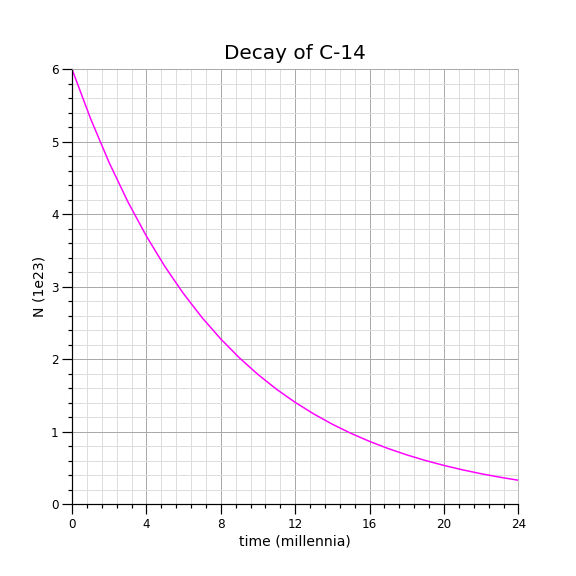
\includegraphics[width=0.9\textwidth,keepaspectratio]{./images/c-14_decay.png}
\caption{Decay curve of C-14}
\end{figure}

Both activity and mass are directly related to the number of nuclei.

\[m = m_0 e^{- \lambda t}\]
\[A = A_0 e^{- \lambda t}\]

\subsubsection{Half-life}
\label{sec:org4fcb785}

Half-life can be linked to the decay constant. When \(t= T_{1/2}\), the number of nuclei remaining is \(N = 0.5N_0\). With these equations, substitutions can be made:


\begin{figure}[H]
\centering
\begin{minipage}{0.8\textwidth}
\begin{tcolorbox}[
sharp corners=all,
colback=white,
colframe=white,
size=tight,
boxrule=0.2mm,
left=10mm, right=10mm,
]
\begin{multicols}{2}
\noindent
\\
\[0.5N_0 = N_0 e^{-\lambda T_{1/2}}\]

\[0.5 = e^{-\lambda T_{1/2}}\]

\[\ln (0.5) = -\lambda T_{1/2}\]

\[-\ln (0.5) = \lambda T_{1/2}\]

\[\textbf{\ldots}\]
\columnbreak
\\
\[\textbf{\ldots}\]

\[\ln (0.5^{-1}) = \lambda T_{1/2}\]

\[\ln (2) = \lambda T_{1/2}\]

\[T_{1/2} = \dfrac{\ln(2)}{\lambda}\]
\\
\\
\end{multicols}
\end{tcolorbox}
\end{minipage}
\end{figure}

\begin{figure}[H]
\centering
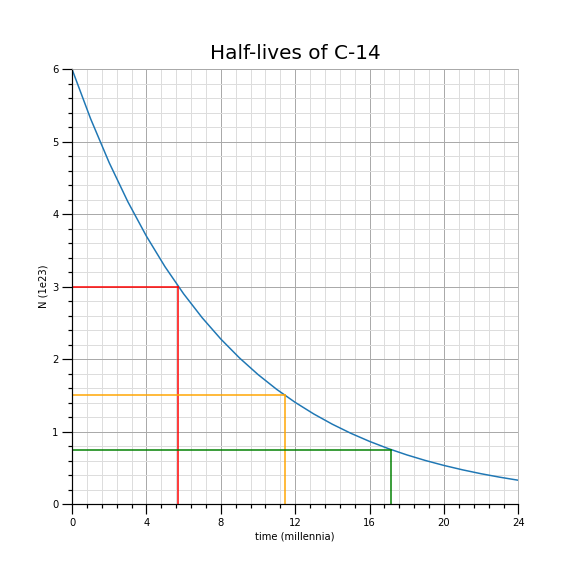
\includegraphics[width=0.9\textwidth,keepaspectratio]{./images/c-14_t_half.png}
\caption{Various half-lives of C-14}
\end{figure}

\subsection{Nuclear Radius}
\label{sec:orgecd71a0}

The radius of a nucleus is proportional to the cube root of the nucleon number and the constant \(r_0\), which is equal to \(1.05fm\).

\[R = r_0 A^{1/3}\]

\[V = \dfrac{4}{3} \pi R^3 = \dfrac{4}{3} \pi (r_0 A^{1/3})^3 = \dfrac{4}{3} \pi {r_0}^3 A\]

Seeing as the mass of a nucleus is equal to \(Au\), where \(u\) is the atomic mass unit, the density of any nucleus is constant.

\[\rho = \dfrac{Au}{4/3 \text{ } \pi {r_0}^3 A} = \dfrac{1u}{4/3 \text{ } \pi {r_0}^3}\]

When evaluated, the density of a nucleus of any element is \(3.4 \times 10^{17}\).

\subsection{Energy and Mass}
\label{sec:orgcac6791}

The equation \(E = mc^2\) links the energy of an object to the change of its mass and the speed of light in free space. Consequently, the mass of any object changes as it gains or loses energy. This is only significant on the nuclear/sub-nuclear scale. The energy released during a reaction is \(Q = \Delta mc^2\), where \(\Delta m\) is the difference in mass before and after the interaction.

\subsection{Binding Energy}
\label{sec:orgb07ff7c}

The binding energy of a nucleus is the work done to separate all of the protons and neutrons from the nucleus. When a nucleus is formed from individual nucleons, energy is released amounting to the binding energy of the nucleus. Due to this release of energy the mass of the nucleus is less than the sum of the masses of constituent nucleons.

The mass defect \(\Delta m\) of a nucleus is the difference between the sum of the masses of separated nucleons and the mass of the whole nucleus. The mass defect for a \(^A_ZX\) nucleus can be calculated with this equation.

\[\Delta m =  Zm_p + (A-Z)m_n - M_{\text{NUC}} \]

Where \(m_p\) and \(m_n\) are the masses of a proton and a neutron respectively and \(M_{\text{NUC}}\) is the mass of the whole nucleus. The binding energy is equal to: \(Q = \Delta mc^2\). The values of \(m_p\) and \(m_n\) are often quoted in terms of \(u\), the atomic mass unit.

\begin{itemize}
\item \(1u = 1.661 \times 10^{-27}kg= 931.3MeV\)
\item \(m_p = 1.00728u\)
\item \(m_n = 1.00867u\)
\end{itemize}

\subsection{Quantum Tunnelling}
\label{sec:orgb724dfa}

Two protons and two neutrons in a nucleus may bind together to as a cluster, which may be ejected from the nucleus as an \(\alpha\) particle. The \(\alpha\) particle is given a large amount of energy during its formation.

\subsection{Nuclear Stability}
\label{sec:org28a7a52}

Each nucleus has a binding energy and a specific binding energy per nucleon. This is the binding energy divided by the nucleon number of the nucleus. This value is indicative of the stability of the nucleus. More stable nuclei have a larger binding energy per nucleon. The maximum value is approximately \(8.7Mev\), occurring in the region \(50 \le A \le 60\).

\begin{figure}[H]
\centering
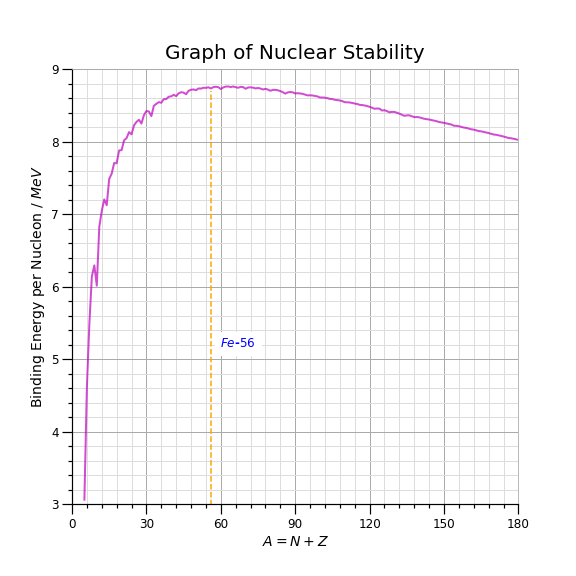
\includegraphics[width=0.9\textwidth,keepaspectratio]{./images/nuclear_stability.png}
\caption{A graph of nuclear stability}
\end{figure}

The orange line in the figure indicates the position of Fe-56, a very stable isotope of Iron. Energy is released in nuclear events under certain conditions:

\begin{itemize}
\item Fusion of nuclei to the left of the division. When heavier nuclei are formed energy is released due to the greater binding energy per nucleon of the resulting nuclei.

\item Fission of nuclei to the right of the division. When multiple, lighter daughter nuclei are formed energy is released due to the greater binding energy per nucleon of the resulting nuclei.
\end{itemize}

\section{Turning Points}
\label{sec:org1dce19b}
\subsection{Discovery of the Electron}
\label{sec:org2fa5f4e}

If a large potential difference is applied across two terminals in an evacuated discharge tube, it is seen glowing in several places. Illustrated in blue in figure \ref{img:cathode_ray} is negative glow, seen when free electrons recombine with positive ions near the negative cathode, causing visible light photons to be released. In the same diagram, the green area represents the glow of the glass container, as cathode rays excite the atoms in the surface which de-excite emitting photons. Between the two terminals, cathode rays may collide with gas atoms, causing excitation and subsequent de-excitation via photon emission.


\begin{figure}[H]
\centering
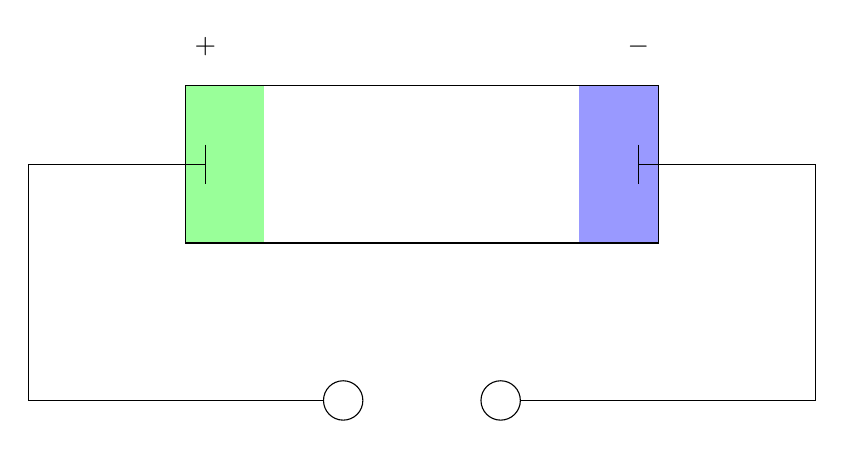
\begin{tikzpicture}
\begin{scope}[very thick,decoration={ markings, mark=at position 0.4 with {\arrow[]{Latex[length=2mm, width=2mm]}}}]
\end{scope}
\fill[blue!40!white] (3,-1) rectangle (2,1);
\fill[green!40!white] (-3,-1) rectangle (-2,1);
\draw (-3,1) -- (3,1) -- (3,-1) -- (-3,-1) -- (-3,1);

\draw (-2.75,0.25) -- (-2.75,-0.25);
\draw (2.75,0.25) -- (2.75,-0.25);

\draw (2.75,0) -- (5,0);
\draw (-2.75,0) -- (-5,0);

\draw (2.75,0) -- (5,0);
\draw (-2.75,0) -- (-5,0);

\draw (-5,0) -- (-5,-3);
\draw (5,0) -- (5,-3);

\node at (-2.75,1.5) {\(+\)};
\node at (2.75,1.5) {\(-\)};

\draw (-5,-3) -- (-1,-3);
\draw (5,-3) -- (1,-3);

\filldraw[fill=white, draw=black] (1,-3) circle (0.25cm);
\filldraw[fill=white, draw=black] (-1,-3) circle (0.25cm);

\end{tikzpicture}
\caption{A glow is seen at the anode due to "cathode rays"}
\label{img:cathode_ray}
\end{figure}

\subsubsection{Electron Guns}
\label{sec:org01e6ee9}

An electron gun is a particle accelerator which transfers energy to the kinetic energy store of electrons by moving them across a potential difference. The electrons are released from the surface of a source, usually wire filament, by thermionic emission.


\begin{figure}[H]
\centering
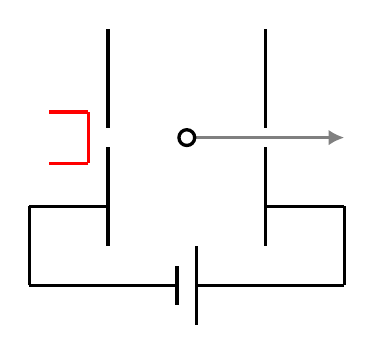
\begin{tikzpicture}
\begin{scope}[very thick,decoration={ markings, mark=at position 0.5 with {\arrow[]{Latex[length=2mm, width=2mm]}}}]
\draw (0.125, -0.5) -- (0.125, 0.5);
\draw (-0.125, -0.25) -- (-0.125, 0.25);
\draw (0.125, 0) -- (2, 0);
\draw (-0.125, 0) -- (-2, 0);
\draw (2, 0) -- (2, 1);
\draw (-2, 0) -- (-2, 1);
\draw (2, 1) -- (1,1);
\draw (-2, 1) -- (-1,1);
\draw (-1, 0.5) -- (-1,1.75);
\draw (1, 0.5) -- (1,1.75);
\draw (-1, 2) -- (-1,3.25);
\draw (1, 2) -- (1,3.25);
\draw[-{Latex[length=2mm, width=2mm]}, gray] (0, 1.875) -- (2, 1.875);
\filldraw[draw=black, fill=white] (0, 1.875) circle (0.1cm);
\draw[red] (-1.25, 1.55) -- (-1.25, 2.2);
\draw[red] (-1.25, 1.55) -- (-1.75, 1.55);
\draw[red] (-1.25, 2.2) -- (-1.75, 2.2);
\end{scope}
\end{tikzpicture}
\caption{Electron Gun}
\end{figure}

The kinetic energy of the emitted electrons is equal to the potential difference (energy per charge) multiplied by the electronic charge. The velocity can also be calculated from the kinetic energy, knowing the electronic mass.

\begin{figure}[H]
\vspace{5mm}
\centering
\begin{minipage}{0.8\textwidth}
\begin{tcolorbox}[
sharp corners=all,
colback=white,
colframe=white,
size=tight,
boxrule=0.2mm,
left=10mm, right=10mm,
]
\begin{multicols}{2}
\noindent
\[\dfrac{1}{2}m_ev^2=eV\]
\columnbreak
\[v=\left ( \dfrac{2eV}{m_e} \right ) ^{1/2}\]
\end{multicols}
\end{tcolorbox}
\end{minipage}
\end{figure}

\subsubsection{Fine Beam Tube}
\label{sec:orgb9291cb}

Using an electron gun, electrons enter a magnetic field at speed. Electrons move in a circular motion as the force due to the field acts at a perpendicular angle to the direction of the beam, providing a centripetal force.

\[F = \dfrac{mv^2}{r} = Bqv\]

\[\dfrac{m_ev^2}{r} = Bev\]

\[\dfrac{m_ev}{r} = Be\]

As the electrons leave the electron gun, their total energy is the product of the potential difference between the anode and cathode and the electronic charge. This value can be used to determine the linear speed of the electrons.


\begin{figure}[H]
\centering
\begin{minipage}{0.8\textwidth}
\begin{tcolorbox}[
sharp corners=all,
colback=white,
colframe=white,
size=tight,
boxrule=0.2mm,
left=10mm, right=10mm,
]
\begin{multicols}{2}
\noindent
\[\dfrac{1}{2}m_ev^2=eV\]

\[v=\left ( \dfrac{2eV}{m_e} \right ) ^{1/2}\]

\[\dfrac{m_e\left ( \dfrac{2eV}{m_e} \right )^{1/2}}{r} = Be\]

\[\textbf{\ldots}\]
\columnbreak
\[\textbf{\ldots}\]

\[\dfrac{m_e2V}{r^2} = B^2e\]

\[\dfrac{e}{m_e} = \dfrac{2V}{r^2  B^2}\]
\\
\\
\end{multicols}
\end{tcolorbox}
\end{minipage}
\end{figure}

\subsubsection{Thomson's Crossed Fields}
\label{sec:org65fc3eb}

A magnetic field is arranged perpendicular to an electric field, so that its force acting on a moving beam of electrons is directly opposing the force on the same beam due to the electric field. The strength of each of these fields are adjusted until the beam of electrons passes through the two fields undeflected; until the two forces are equal and opposite.


\begin{figure}[H]
\centering
\begin{minipage}{0.8\textwidth}
\begin{tcolorbox}[
sharp corners=all,
colback=white,
colframe=white,
size=tight,
boxrule=0.2mm,
left=10mm, right=10mm,
]
\begin{multicols}{2}
\noindent
\[F = Eq = Bqv\]

\[E = V/d\]

\[\dfrac{Ve}{d} = Bev\]

\[\textbf{\ldots}\]
\columnbreak
\[\textbf{\ldots}\]

\[v = \dfrac{Ve}{Bd}\]

\[\dfrac{1}{2}m_ev^2=eV_a\]

\[\dfrac{e}{m_e} = \dfrac{V^2}{2B^2d^2V_a}\]

\end{multicols}
\end{tcolorbox}
\end{minipage}
\end{figure}

This particular method is significant as it demonstrates that the properties of the electrons are the same no matter which gas they emitted from, therefore it can be concluded that all atoms contain electrons. The specific charge of electrons is about 1800 times higher than that of a proton.

\subsection{Wave Particle Duality}
\label{sec:org1205059}
\subsection{Discovery of EM Waves}
\label{sec:org782b4d3}

Maxwell theorised that EM waves travelled at speed \(c\) in a vacuum, without any experimental evidence.

\[c = \dfrac{1}{({\mu}_0 {\epsilon}_0)^{1/2}}\]

\subsection{Special Relativity}
\label{sec:org5c17630}
\subsubsection{Interferometer}
\label{sec:orge630f37}

Scientists Michelson and Morley designed an interferometer, a device used to measure the speed of the earth through the ether. Using a partially reflective half-silvered mirror, a light source is split into two arms, which are perpendicular to each other. One of these beams may be sent through a compensating glass block, so that both beams travel through the same amount of material. Each of those light beams is reflected back toward the mirror, where they are superposed on one another.  The resulting interference pattern is directed towards a detector.



\begin{figure}[H]
\centering
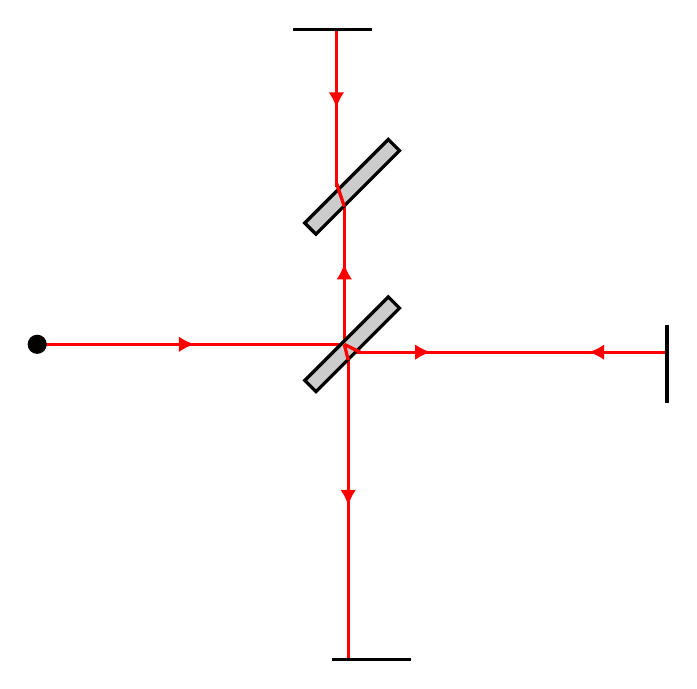
\begin{tikzpicture}
\begin{scope}[very thick,decoration={ markings, mark=at position 0.5 with {\arrow[]{Latex[length=2mm, width=2mm]}}}]
\draw[color=red, postaction={decorate}] (-4, 0) -- ( 0, 0);
\draw[color=red, postaction={decorate}] (-0.1, 0.05) -- (-0.1, 2);
\draw[color=red, postaction={decorate}] (-0.2, 4) -- (-0.2, 2);
\draw[color=red, postaction={decorate}] (0, -0.1) -- (2, -0.1);
\draw[color=red, postaction={decorate}] (4, -0.1) -- (2, -0.1);
\draw[color=red, postaction={decorate}] (-0.05, -0.1) -- (-0.05, -4);
\draw (-0.75, 4) -- (0.25, 4);
\draw (4, 0.25) -- (4, -0.75);
\draw (-0.25, -4) -- (0.75, -4);
\filldraw[fill=black, draw=black] (-4,0) circle (0.1cm);
\filldraw[fill=black!20!white,  draw=black, rotate around={45:(0,0)}] (-0.75,-0.1) rectangle (0.75,0.1);
\filldraw[fill=black!20!white,  draw=black, rotate around={45:(0,2)}] (-0.75,1.9) rectangle (0.75,2.1);

\draw[color=red] (-0.1, 0) -- (0.1, -0.1);
\draw[color=red] (-0.1, 1.75) -- (-0.2, 2.05);
\draw[color=red] (-0.05, -0.2) -- (-0.1, 0);

\end{scope}
\end{tikzpicture}
\caption{The Michelson-Morley interferometer}
\end{figure}

It was believed that the light travelling parallel in the direction of earth would be affected and hence take longer to travel. This would not affect the path of the light beam perpendicular to the earth's motion. When the apparatus was rotated through 90 degrees no change in the interference pattern was observed. This proved that the rotation of the system did not affect the speed that light travelled.

These observations disproved the existing understanding of absolute motion. Either the ether did not exist, or moved with the earth, or the speed of light in free space is invariant.

\subsubsection{Black Body}
\label{sec:org323a78a}

A black body is an idealised system which absorbs all incident electromagnetic radiation, regardless of its frequency or angle of incidence. Black bodies are often modelled as a sealed insulated container, with sides impermeable to radiation and a small whole, through which incident radiation is absorbed. After some time all energy absorbed by a black body is emitted as black body radiation.

In order to remain in thermal equilibrium, they system will radiate energy characteristic of this system, not necessarily the type of radiation incident on it. The radiated energy can be considered to be produced by standing wave or resonant modes of the cavity which is radiating. The density of modes, the number of modes per unit frequency per unit volume, is expressed as:

\[\dfrac{8 \pi f^2}{c^3}\]

A classical interpretation of wave theory, devised by Rayleigh and Jeans, linked the intensity of radiation at a given frequency and temperature to \(f^2\). This expression would suggest that the intensity of radiation would rise dramatically at high frequencies, leading to a situation described as the \emph{ultraviolet catastrophe}.

\[ u(f, T) = \dfrac{8 \pi f^2}{c^3}kT\]

The quantised theory of EM waves addressed this issue, with an expression that applied to all frequencies of radiation.

\[ u(f, T) = \dfrac{8 \pi f^2}{c^3} \dfrac{hf}{e^{hf/kT} - 1}\]

\subsubsection{Einstein's Theory of Special Relativity}
\label{sec:org9228b7a}

An inertial frame of reference is not undergoing acceleration, it is at constant velocity. Einstein's theory of special relativity applies to these frames of reference with certain assumptions, called \emph{postulates}. The first postulate is that the speed of light in free space is invariant. The second is that the laws of physics are the same in all inertial frames of reference.

\subsubsection{Time Dilation}
\label{sec:orga4cd6e4}

A consequence of special relativity, time dilation is the difference in elapsed time between a stationary and external observer to a frame of reference. The frame of reference is reference appears in motion to an external observer.

The time measured to have passed by the stationary observer is the proper time, \(t_0\). The time measured by an external observer, \(t\), is always larger than proper time and is calculated:

\[t = \dfrac{t_0}{\sqrt{1 - \dfrac{v^2}{c^2}}}\]

\subsubsection{Length Contraction}
\label{sec:orgabdc291}

A consequence of special relativity, length contraction applies to inertial frames of reference and causes the lengths of objects at speed to appear shorter. The length of an object as seen bu an observer


\[l = l_0\sqrt{1 - \dfrac{v^2}{c^2}}\]

\subsubsection{Mass \& Energy}
\label{sec:org4111710}

Mass and Energy are proven to be interchangeable, according to \(E=mc^2\). Supplying more energy to an object will increase its mass, therefore the mass of an object increases at speed. Resulting values of mass are the \emph{relativistic mass}, \(m\).


\[m = \dfrac{m_0}{\sqrt{1 - \dfrac{v^2}{c^2}}}\]

When a mass moves at relativistic speeds (over a tenth of the speed of light), its mass will increase significantly and hence \(1/2mv^2\) is no longer a suitable expression for kinetic energy. The kinetic energy of a mass in relativistic motion is the total energy less the rest mass of the object, \(m_0\).

\[E_T = E_K + E_0\]

\[E = \dfrac{m_0c^2}{\sqrt{1 - \dfrac{v^2}{c^2}}}\]

\[E_K = \dfrac{m_0c^2}{\sqrt{1 - \dfrac{v^2}{c^2}}} - m_0c^2\]
\end{document}
